\documentclass[]{article}
\usepackage{amsmath}
\usepackage{amsfonts}
\usepackage{amssymb}

\usepackage[utf8]{inputenc}
\usepackage[T1]{fontenc}

\usepackage{graphicx}
\graphicspath{{./graphs/}}
\usepackage{float}

%opening
\title{
	{\large Sprawozdanie do zadania pierwszego}\\
	{\LARGE Badanie złożoności obliczeniowej algorytmów sortujących}}
\author{Piotr Tylczyński, Bartosz Pilarczyk}
\date{21.03.2019}

\begin{document}

\maketitle

\section{Sortowaine przez wybór}
	\subsection{Opis}
		Typ sortowania stabilnego polegający na wyborze najmniejszego elementu spośród elementów nie posortowanych i wstawienie go tuż za ostatnim posortowanym elementem. Taka implementacja pozwala na sortowanie elementów zbioru w porządku rosnącym. Dla przypadku odwrotnego, czyli sortowania w porządku malejącym należy zamiast najmniejszego elementu wybierać element najwiękysz. Algoryt pozwala na implementację insitu, czyli sortowania w miejscu. Sprawia to, że wykonanie algorytmu nie wymaga tworzenia nowych struktór danych przetrzymujących sortowane dane w czasie sortowania
	\subsection{Złożoność czasowa}
		Algorytm charakteryzuję się złożonością czasową na poziomie
		\[
			O(n^2)
		\]
		Jest to spowodowane potrzebą ciągłego wyszukiwania najmniejszego/największego elementu w zbiorze. Ta operacja wymaga wykonania k operacji, gdzie k jest ilością elementów  w zbiorze. Dokładną ilość operacji kluczowych można wyliczyć ze wzoru
		\[
			\text{ilość operacji} = \sum_{i = 1}^{n - 1}{i}
		\]
		co daje wyżej wymienioną złożoność.
		Sprawia to, że jest to algorytm skrajnie nieefektywny dla dużych struktur danych. Jest to jedna z najgorszych złożoności czasowych testowanych przez nas algorytmów. Łatwo zauważyć, że podczas sortowania powyżej 1000 elementów następuje nagłę wydłużenie czasu wykonania. Natomiast jego zdecydowaną zaletą jest prostota implementacji i małe zużycie dodatkowej pamięci.
		
	 	
	\subsection{Efektywność algorytmu, a wstępne uporządkowania danych}
		\begin{figure}[H]
			\centering
			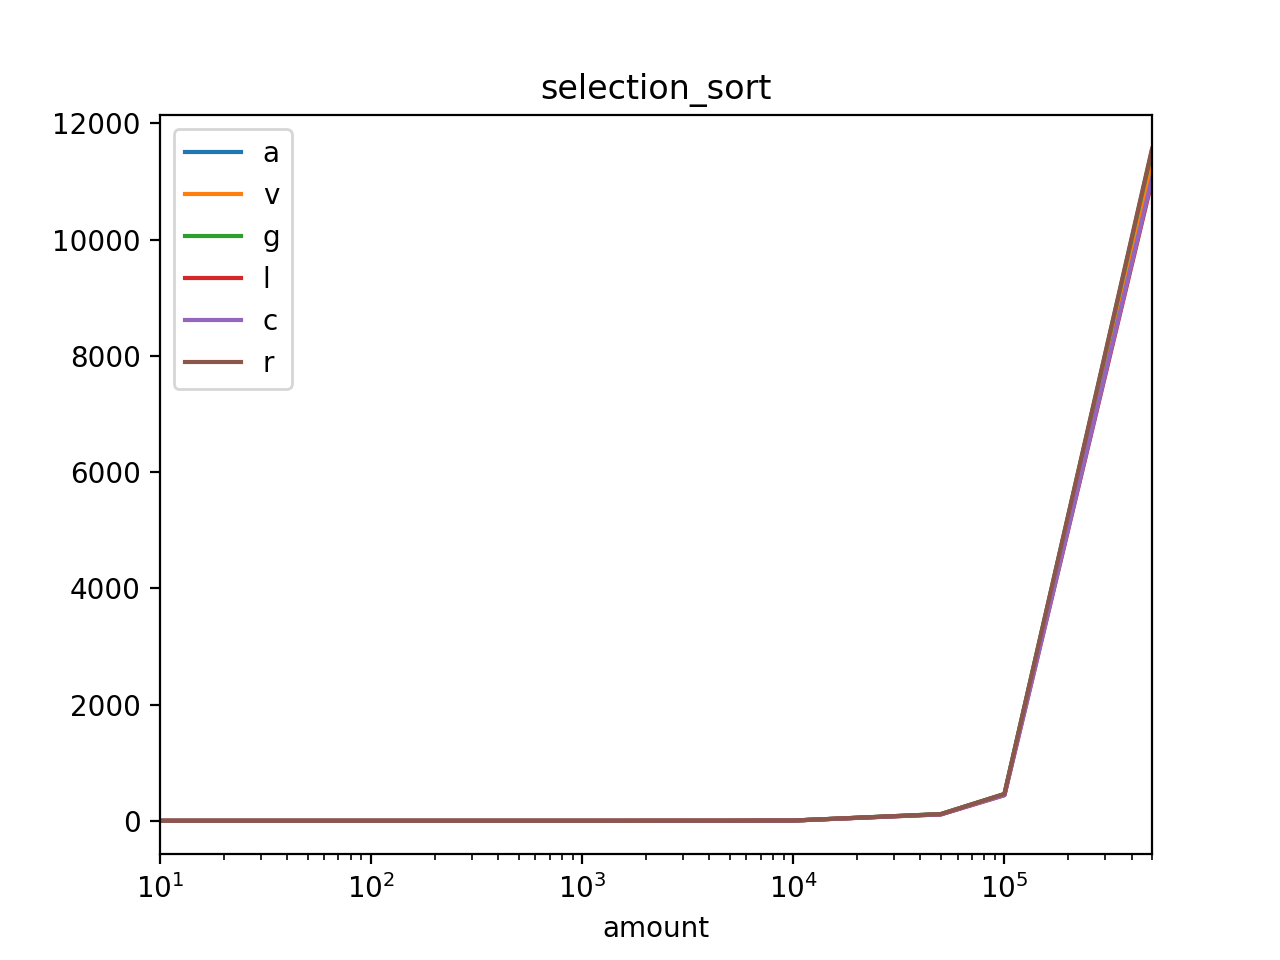
\includegraphics[width=8cm]{selection_sort_gather.png}	
		\end{figure}
		Poniżej zaprezentowano czasy wykonania sortowania w zależności od ilości elementów i ich uporządkowania. Dla wykresów zastosowano skalę logarytmiczną ze względu na znaczące różnice w czasie wykonania algorytmów. Nietrudno zauważyć, że czas potrzebny na posortowanie zbioru danych nie zależy od tego jak ułożone są dane. Jest to spowodowane potrzebą każdorazowego przeglądania nieuporządkowanej części zbioru w celu znalezienia elementu najmniejszego. Na czas przeszukania zbioru nie ma wpływu to jak są ułożone w nim dane, a to powoduje, brak wpływu uporządkowania danych na ogólny czas wykonania algorytmu.
		\subsubsection{Uporządkowanie rosnąco-malejące}
			\begin{figure}[H]
				\centering
				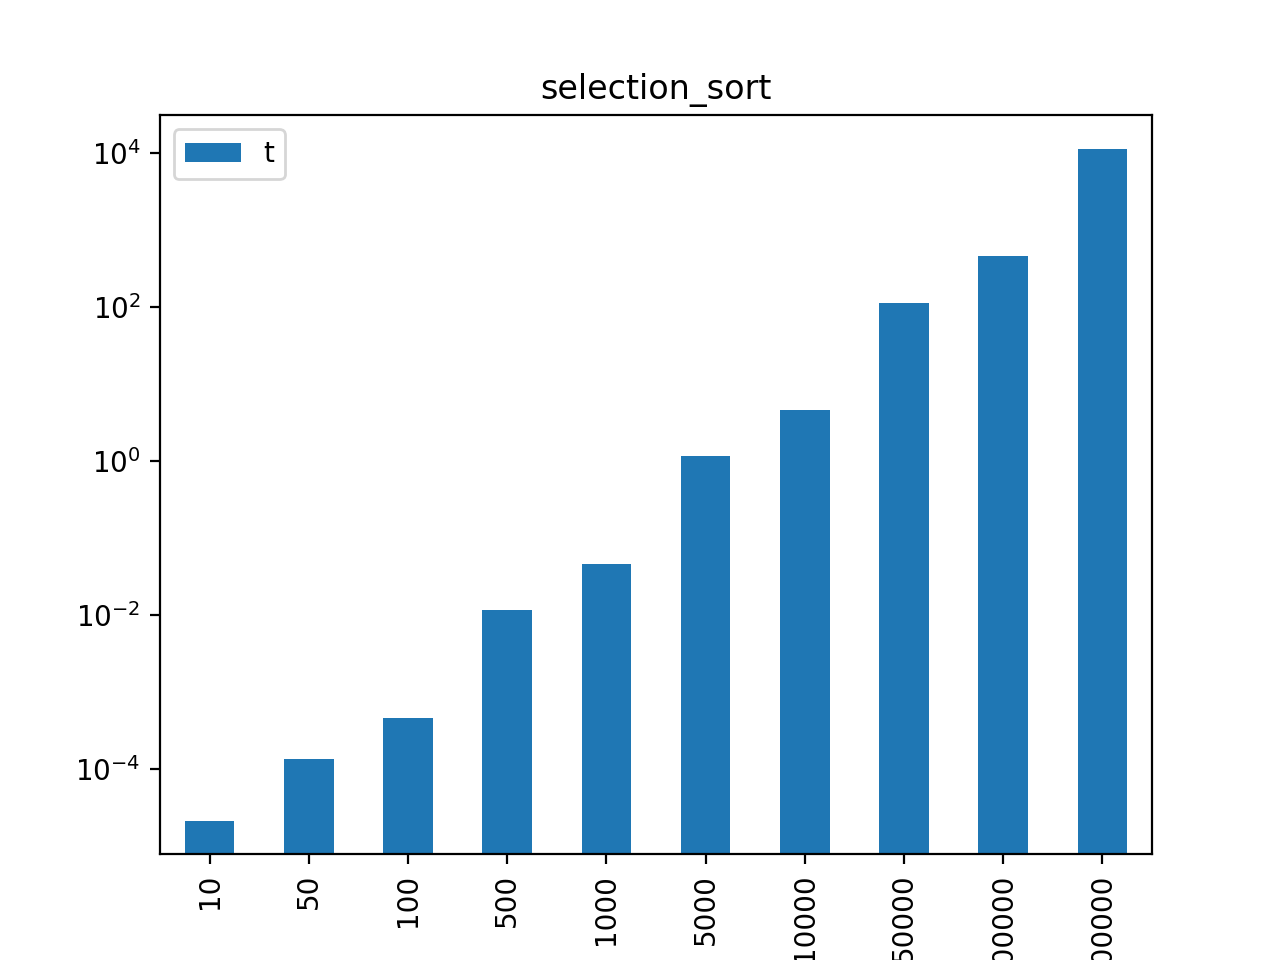
\includegraphics[width=8cm]{selection_sort_a.png}	
			\end{figure}
		\subsubsection{Uporządkowanie malejąco-rosnące}
			\begin{figure}[H]
				\centering
				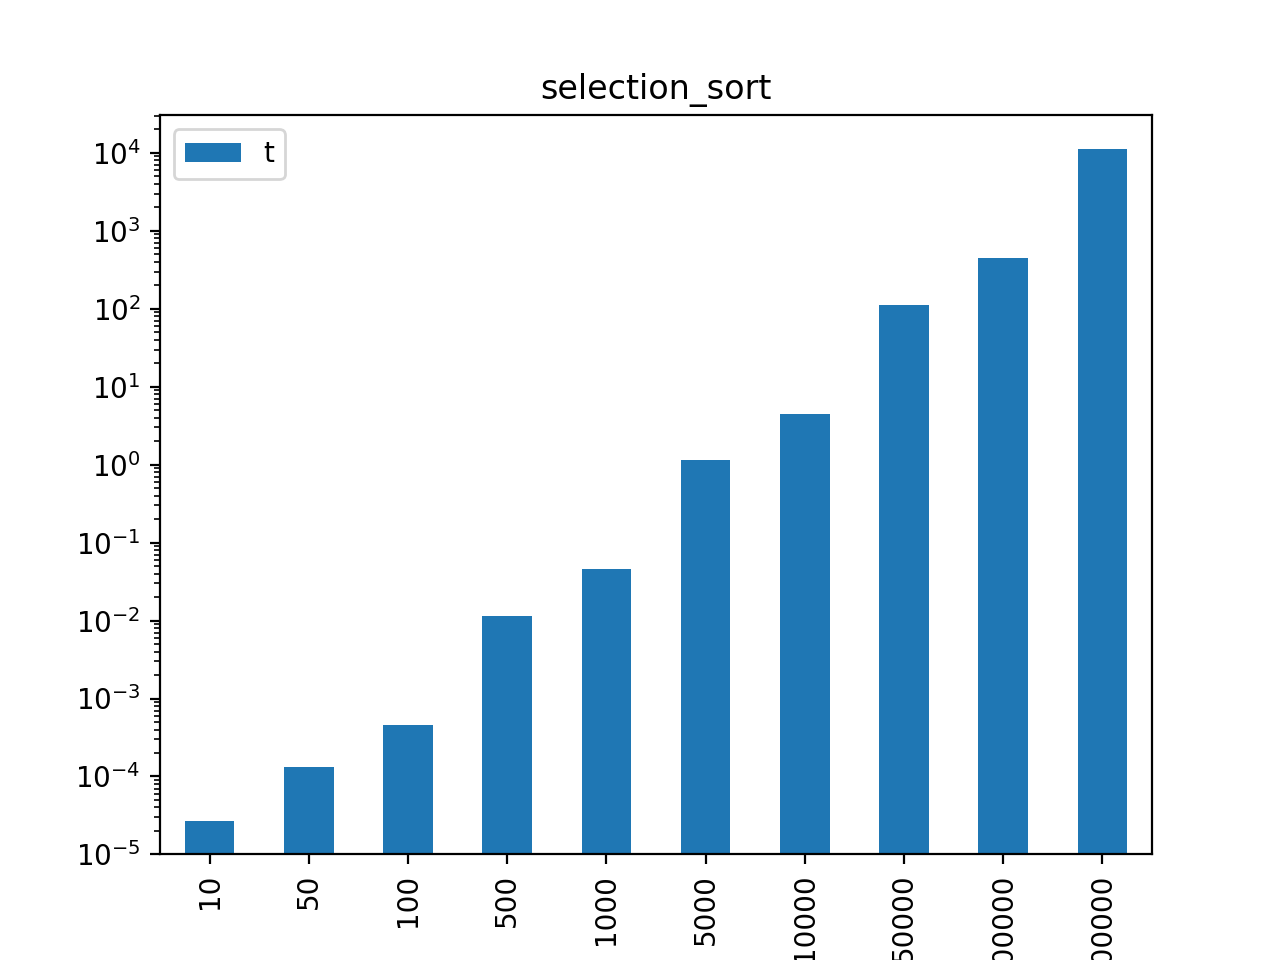
\includegraphics[width=8cm]{selection_sort_v.png}	
			\end{figure}
		\subsubsection{Uporządkowanie rosnące}
			\begin{figure}[H]
				\centering
				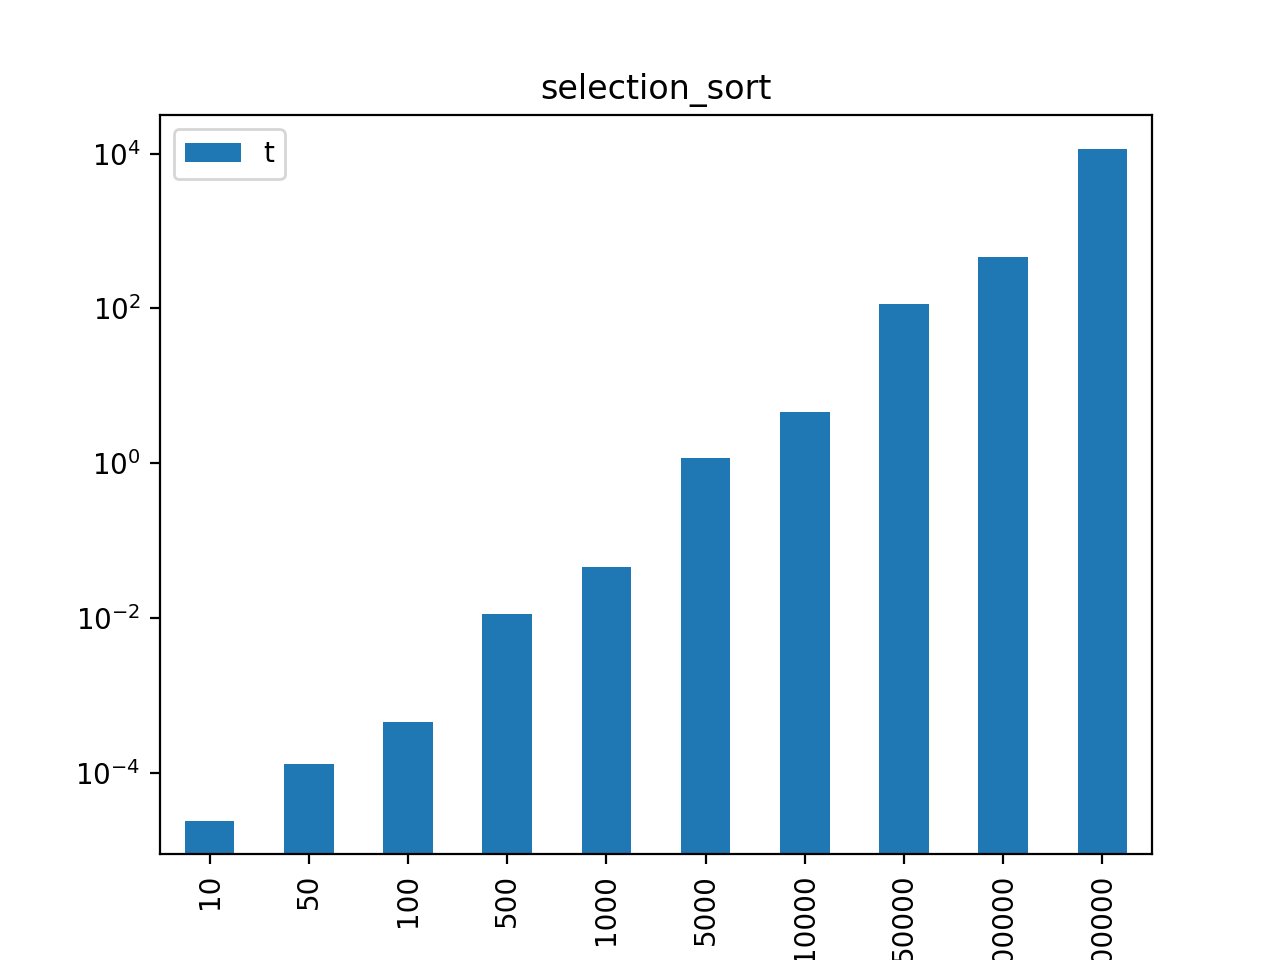
\includegraphics[width=8cm]{selection_sort_g.png}	
			\end{figure}
		\subsubsection{Uporządkowanie malejące}
			\begin{figure}[H]
				\centering
				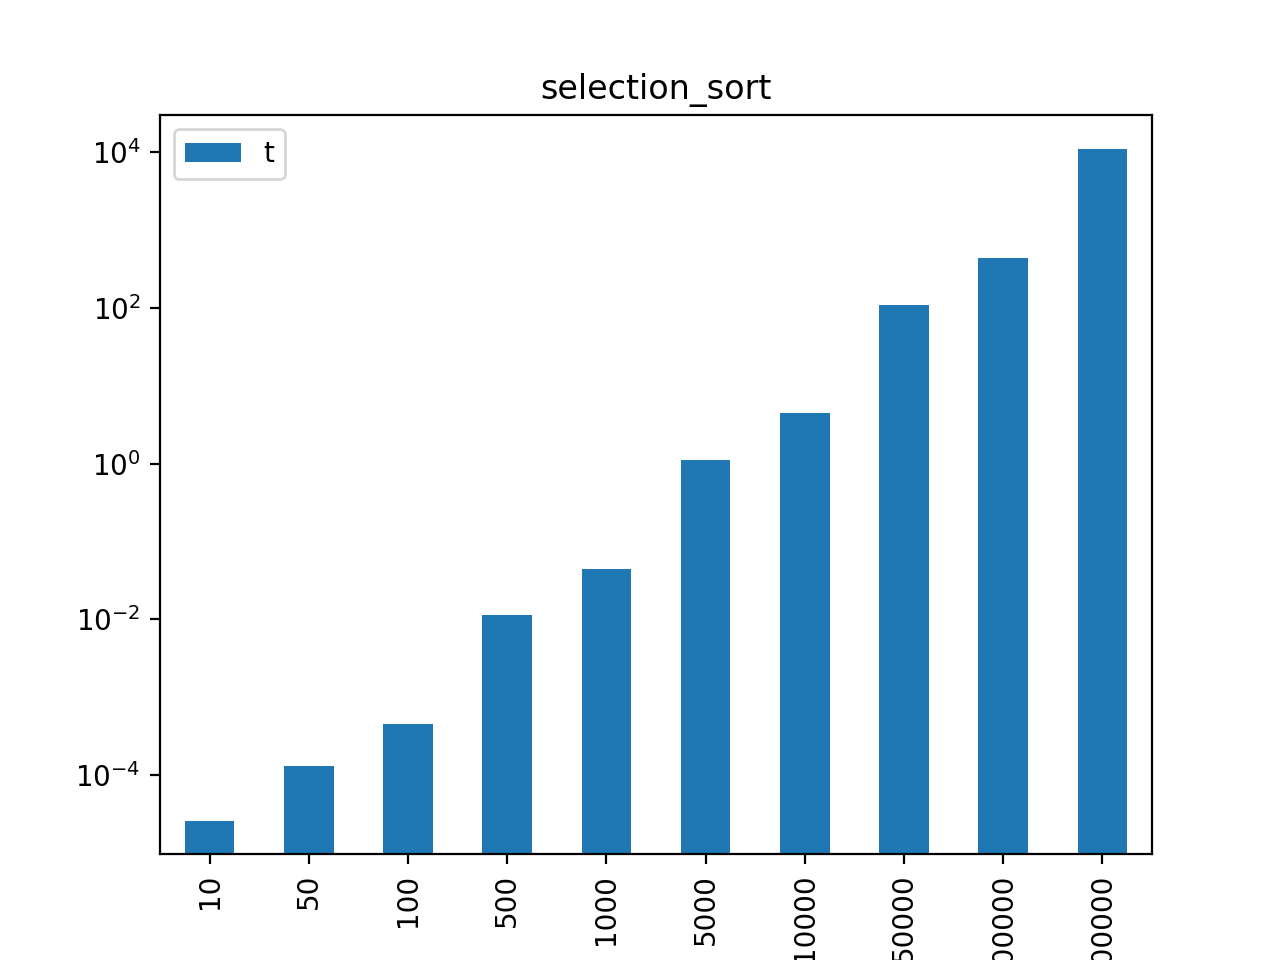
\includegraphics[width=8cm]{selection_sort_l.png}	
			\end{figure}
		\subsubsection{Wszystkie elementy są sobie równe}
			\begin{figure}[H]
				\centering
				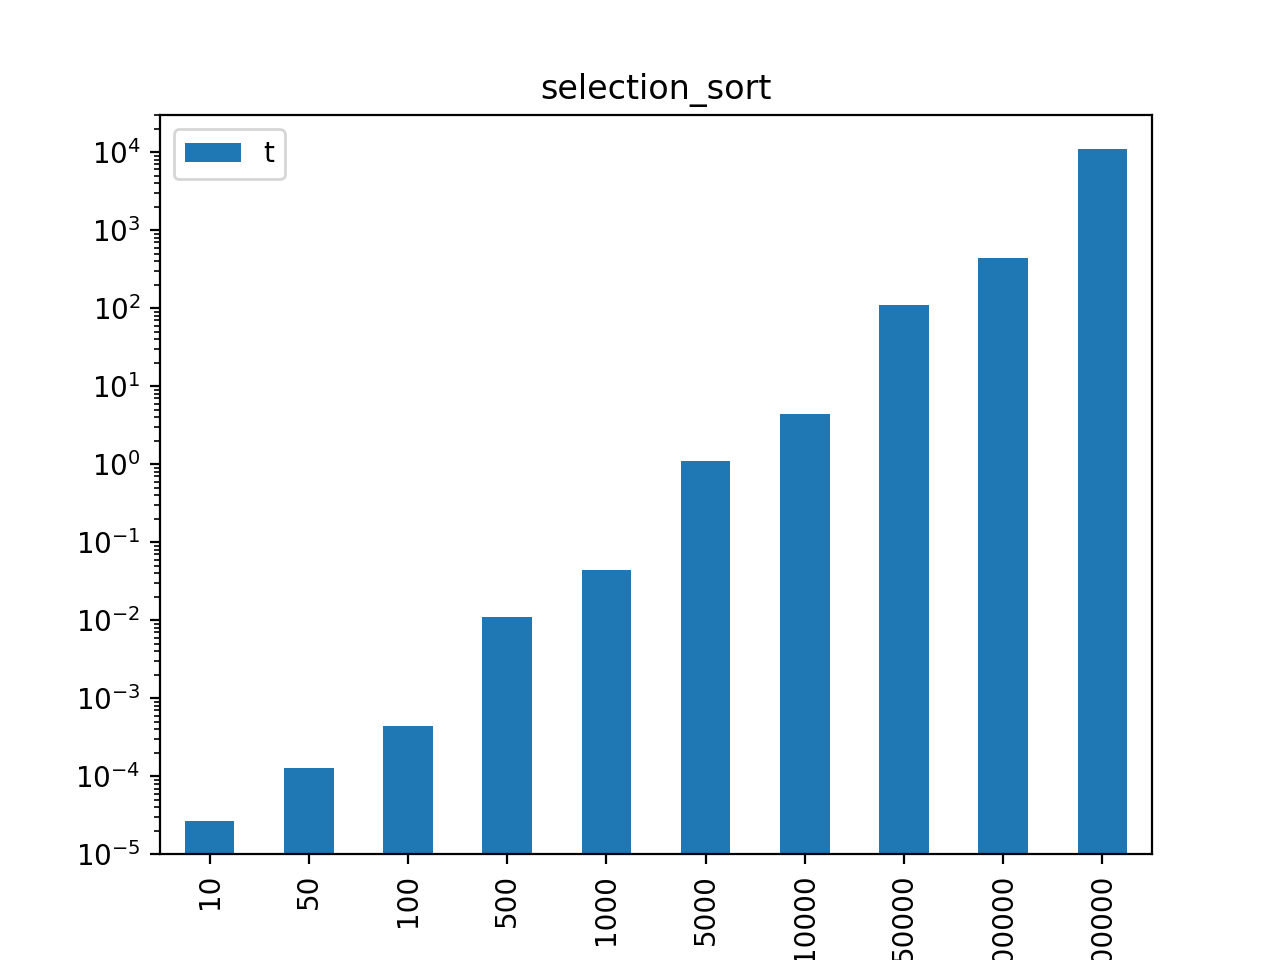
\includegraphics[width=8cm]{selection_sort_c.png}	
			\end{figure}
		\subsubsection{Brak wstępnego uporządkowania}
			\begin{figure}[H]
				\centering
				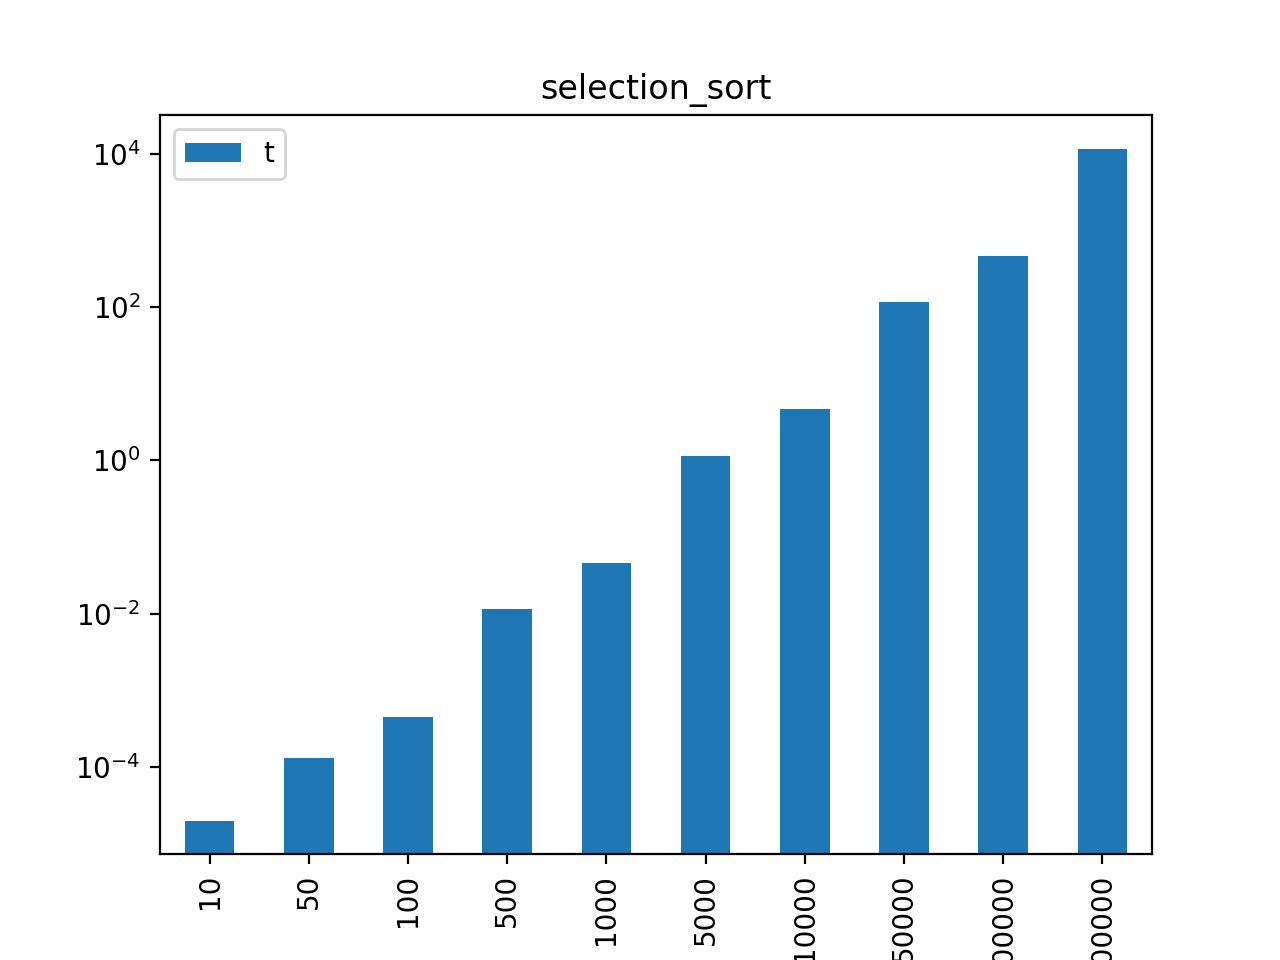
\includegraphics[width=8cm]{selection_sort_r.png}	
			\end{figure}
\pagebreak
\section{Sortowaine przez wstawianie}
	\subsection{Opis}
		Jest to typ sortowania stabilnego polegający na wstawianiu kolejnych elementów z nieposortowanej części zbioru do posortowanej części zbioru. Jest to kolejny algorytm pozwalający na sortowanie insitu, co pozwala na nie wykorzystywanie dodatkowych struktur danych podczas sortowania.
	\subsection{Złożoność czasowa}
		Algorytm posiada złożoność czasową
		\[
		O(n^2)
		\]
		Jednak, złożoność ta może stać się lepsza dla niektórych przypadków ułożeń danych (co zostało omóione w dalszej części). Ilość operacji elementarnych wykonanych przez algorytm, w najgorszym przypadku, można obliczyć ze wzoru
		\[
		\text{ilość obliczeń} = \sum_{n - 1}^{i = 1}i
		\]
		ponieważ, jeżeli każdy element z nieposortowanej części zbioru, będzie mniejszy niż wszystkie pozostałe elementy w posortowanej części zbioru, to algorytm będzie musiał porównać sortowany element ze wszystkimi elementami w posortowanej części zbioru, zanim przekona się, że sortowany element jest faktycznie najmniejszy
	\subsection{Efektywność algorytmu, a wstępne uporządkowania danych}
		\begin{figure}[H]
			\centering
			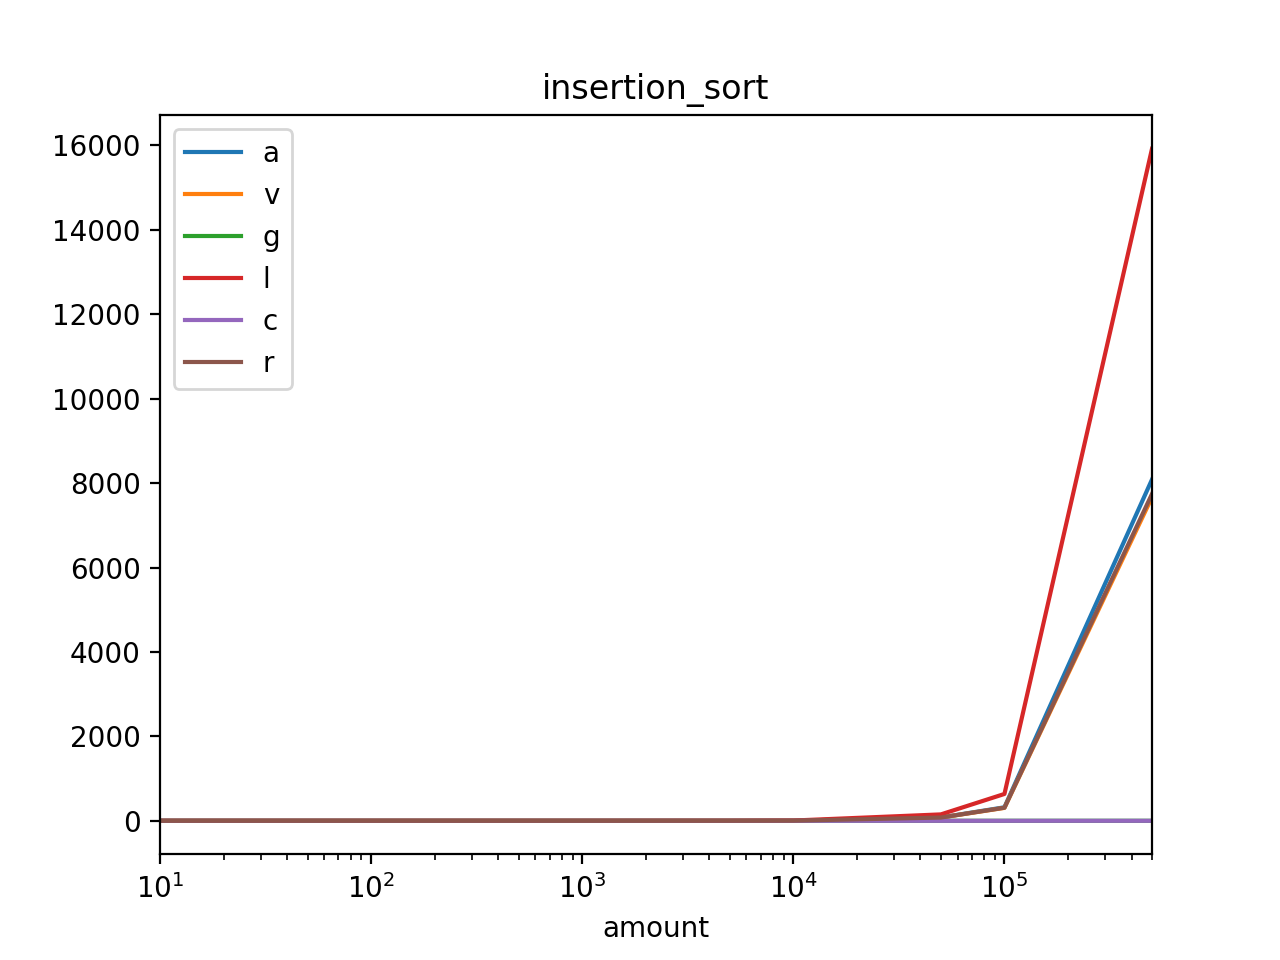
\includegraphics[width=8cm]{insertion_sort_gather.png}	
		\end{figure}
		\subsubsection{Uporządkowanie rosnąco-malejące}
			\begin{figure}[H]
				\centering
				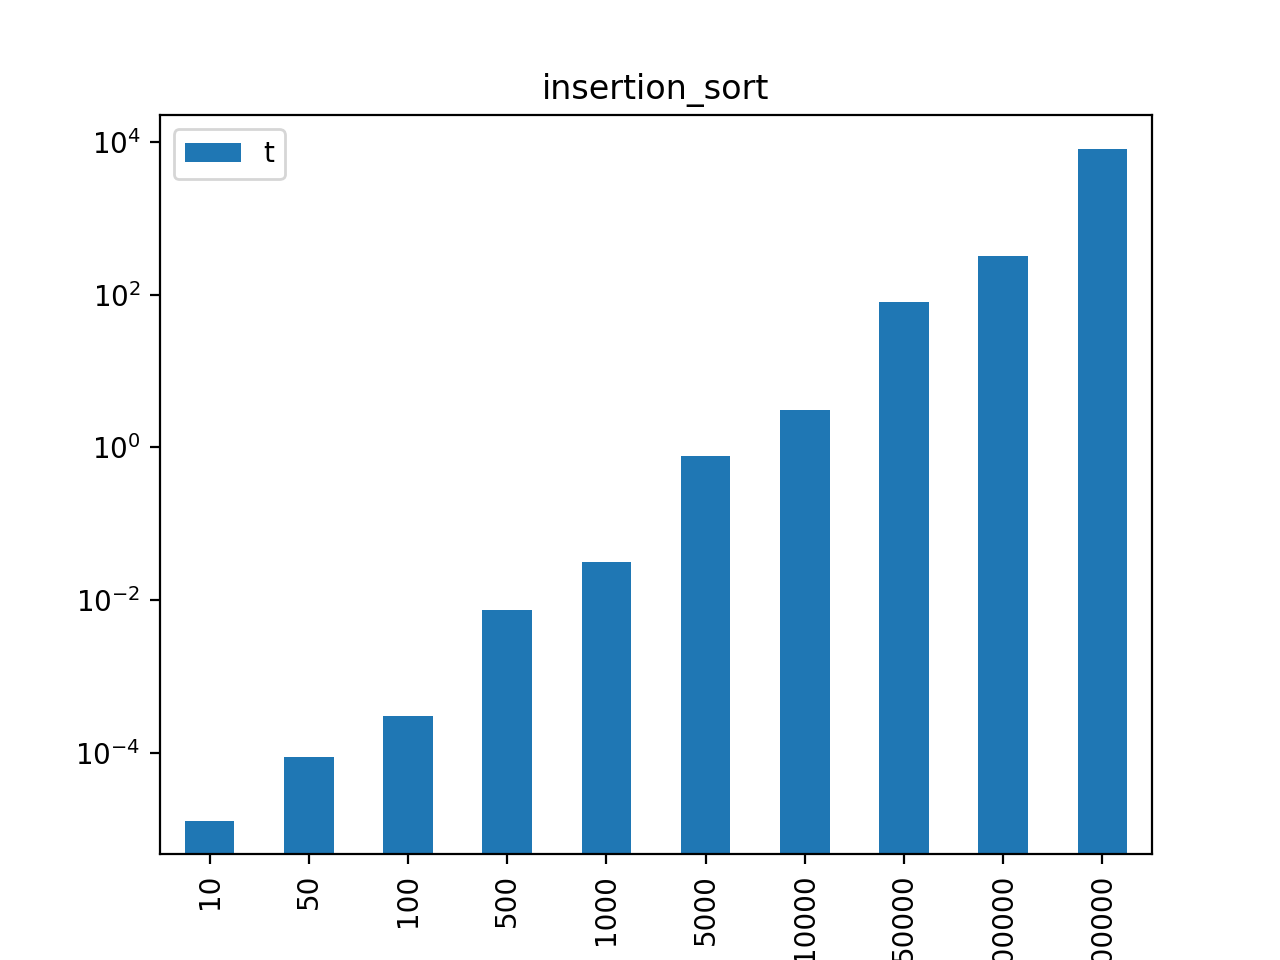
\includegraphics[width=8cm]{insertion_sort_a.png}	
			\end{figure}
			Pierwsza część danych jest już wstępnie posortowana, dlatego algorytm wykonuję się szybko. Dokładne wytłumaczenie dlaczego algorytm jest szybki dla uporządkowanych danych, znajduję się poniżej. Natomiast druga część danych, wymaga posortowania, które jest najgorszym możliwym przypadkiem - dane są ułożone w sposób malejący, a algorytm sortuje w sposób rosnący. Z tego powodu łatwo zauważyć, że czas wykonania jest połową czsu wykonania potrzebengo dla posortowania zbioru ułożonego w sposób malejący, który jest najgorszym do sortowania przypadkiem. 
			\subsubsection{Uporządkowanie malejąco-rosnące}
			\begin{figure}[H]
				\centering
				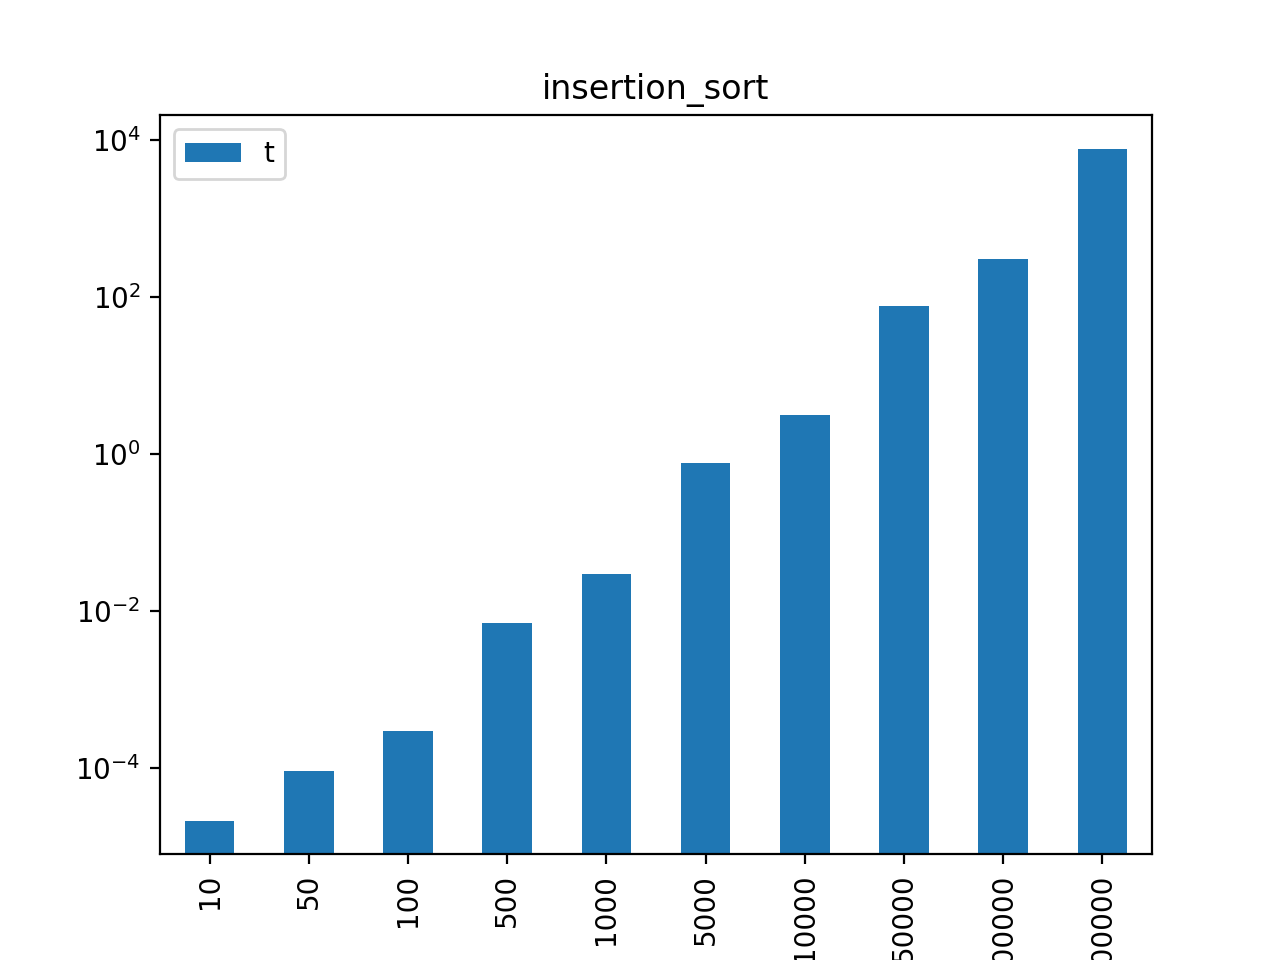
\includegraphics[width=8cm]{insertion_sort_v.png}	
			\end{figure}
			W przypadku takie ułożenia danych, można zauważyć analogię do wyżej opisanego przypadku. Jest to spowodowane tym, że pierwszą część danych należy posortować a pozostałą tylko dopisać w odpowiednie miejsca
		\subsubsection{Uporządkowanie rosnące}
			\begin{figure}[H]
				\centering
				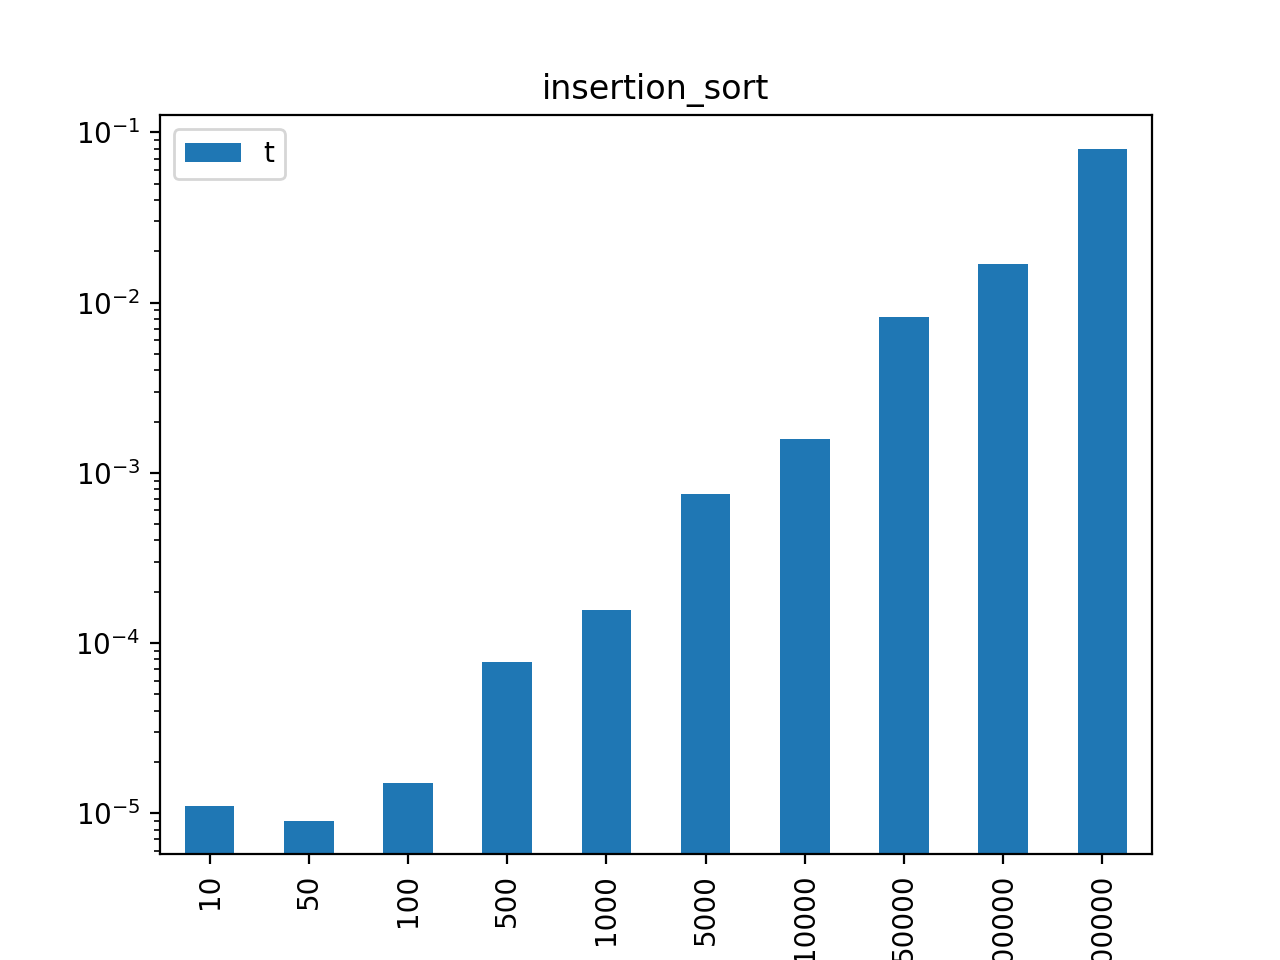
\includegraphics[width=8cm]{insertion_sort_g.png}	
			\end{figure}
			Dla uporządkowania rosnącego algoprytm sortowania przez wstawianie wykonuję się szybko. W takim wypadku jego złożoność jest opisywana przez $ O(n) $, ponieważ algorytm dla każdego kolejnego elementu z zbioru nieposortowanego, nie musi szukać miejsca w posortowanej części zbioru, gdyż ten element już znajduje się na swoim miejscu
		\subsubsection{Uporządkowanie malejące}
			\begin{figure}[H]
				\centering
				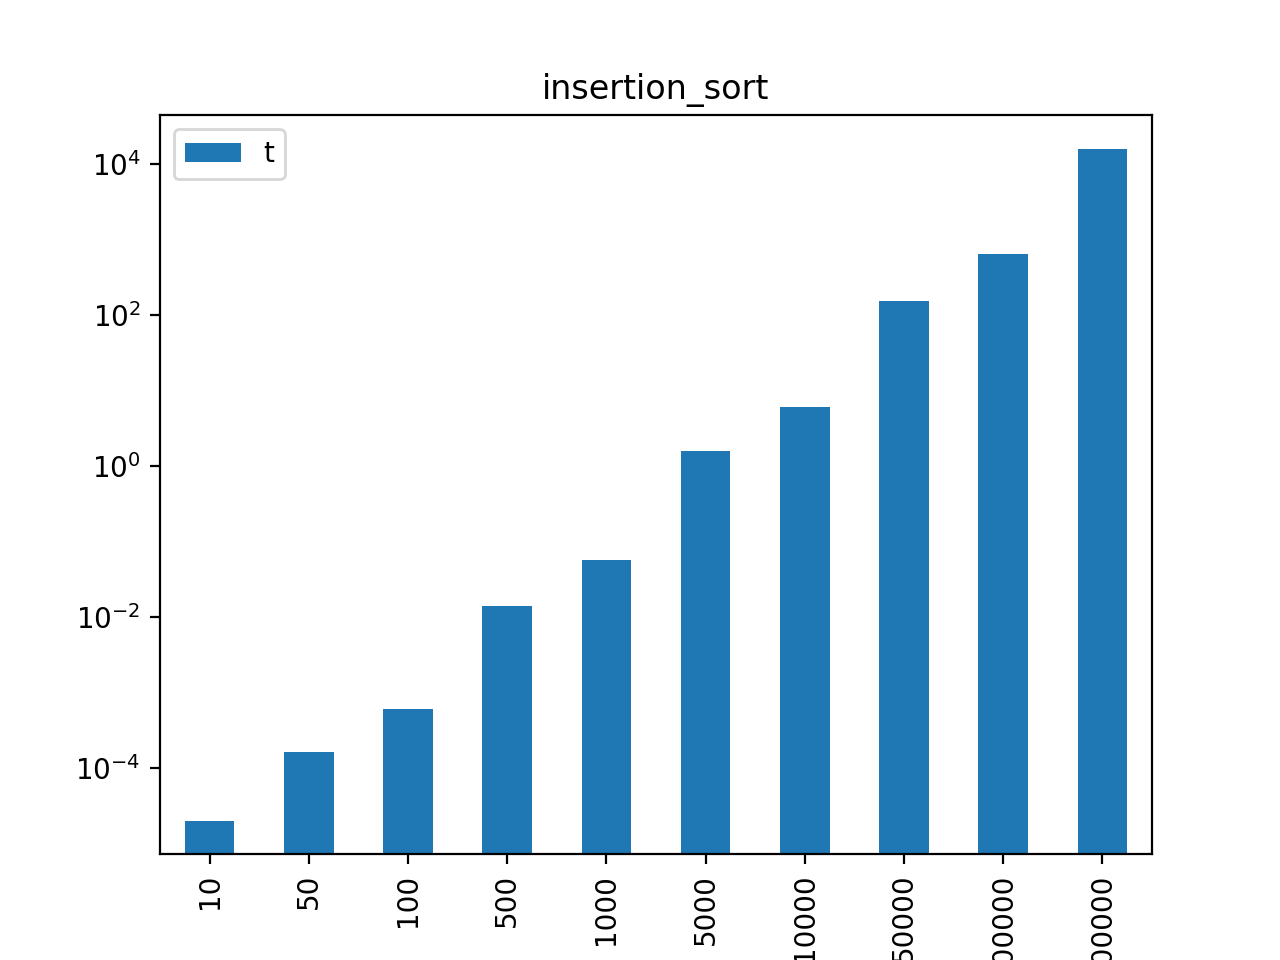
\includegraphics[width=8cm]{insertion_sort_l.png}	
			\end{figure}
			Jest to przypadek zdecydowanie najgorszy, ponieważ każdy element z zbioru nieuporządkowanego jest najmniejszy ze wszystkich elementów w zbiorze już uporządkowanym, dlatego należy go porównać ze wszystkimi elementami w zbiorze posortowanym.
		\subsubsection{Wszystkie elementy są sobie równe}
			\begin{figure}[H]
				\centering
				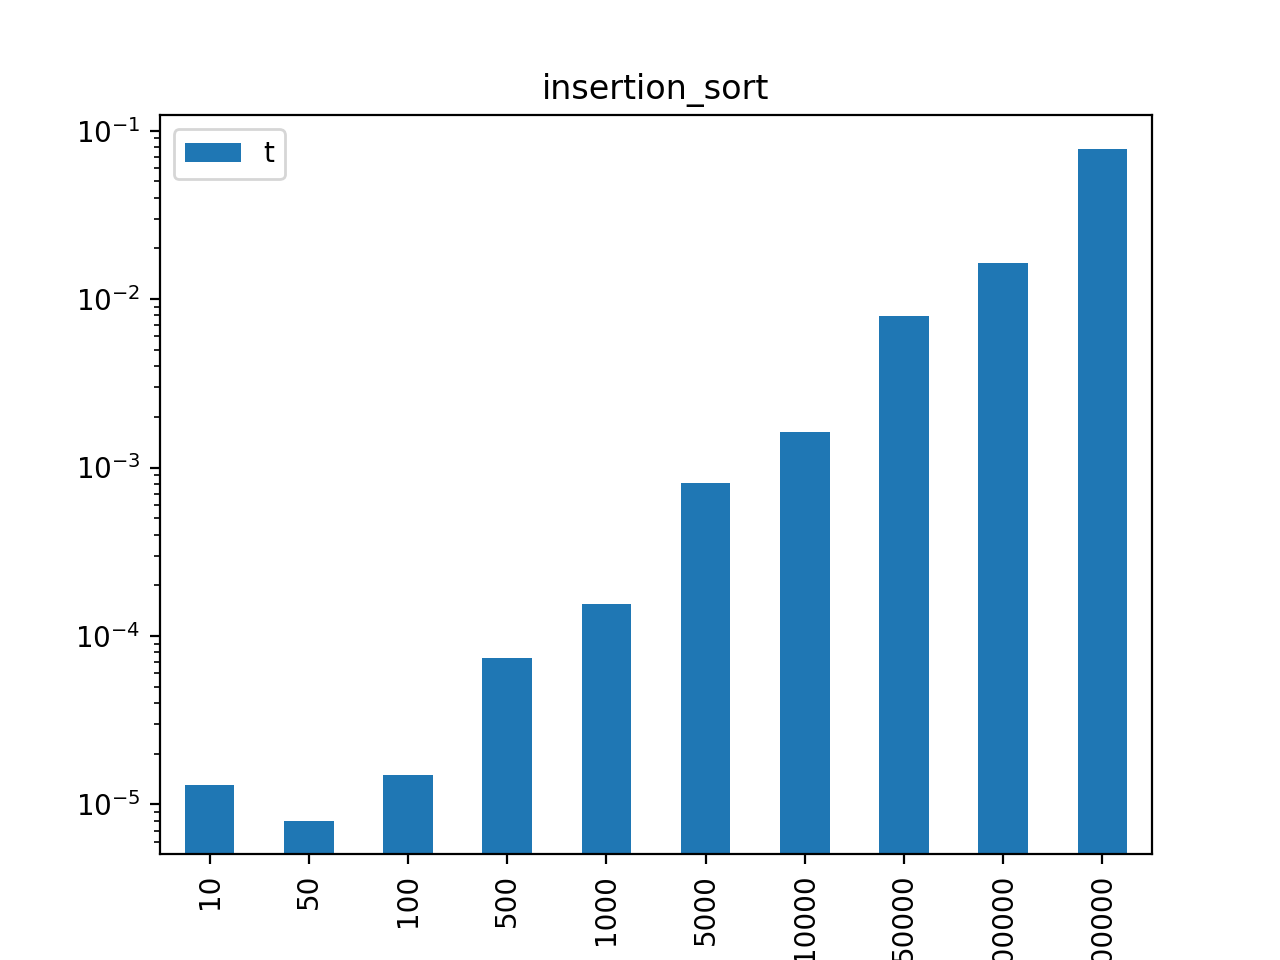
\includegraphics[width=8cm]{insertion_sort_c.png}	
			\end{figure}
			Jest to przypadek analogiczny do wstępnego posortowania rosnącego. Poprawnie zaimplementowny algorytm wykona się ze złożonością liniową, ponieważ będzie zauważał, że każdy kolejny z elemntów w zbiorze nieposortowanym jest równy pierwszemu elementowi ze zbioru uporządkowanego, a przez to nie wykonywał następnych porównań. Jednak istnieje możliwość implementacji, w której algorytm po znaleziemiu w zbiorze posortowanym, elemntu równego będzie szukał kolejnych elementów do momentu kiedy nie znajdzie elementu mniejszego. W takim przypadku algorytm będzie miał złożoność $ O(n^2) $
		\subsubsection{Brak wstępnego uporządkowania}
			\begin{figure}[H]
				\centering
				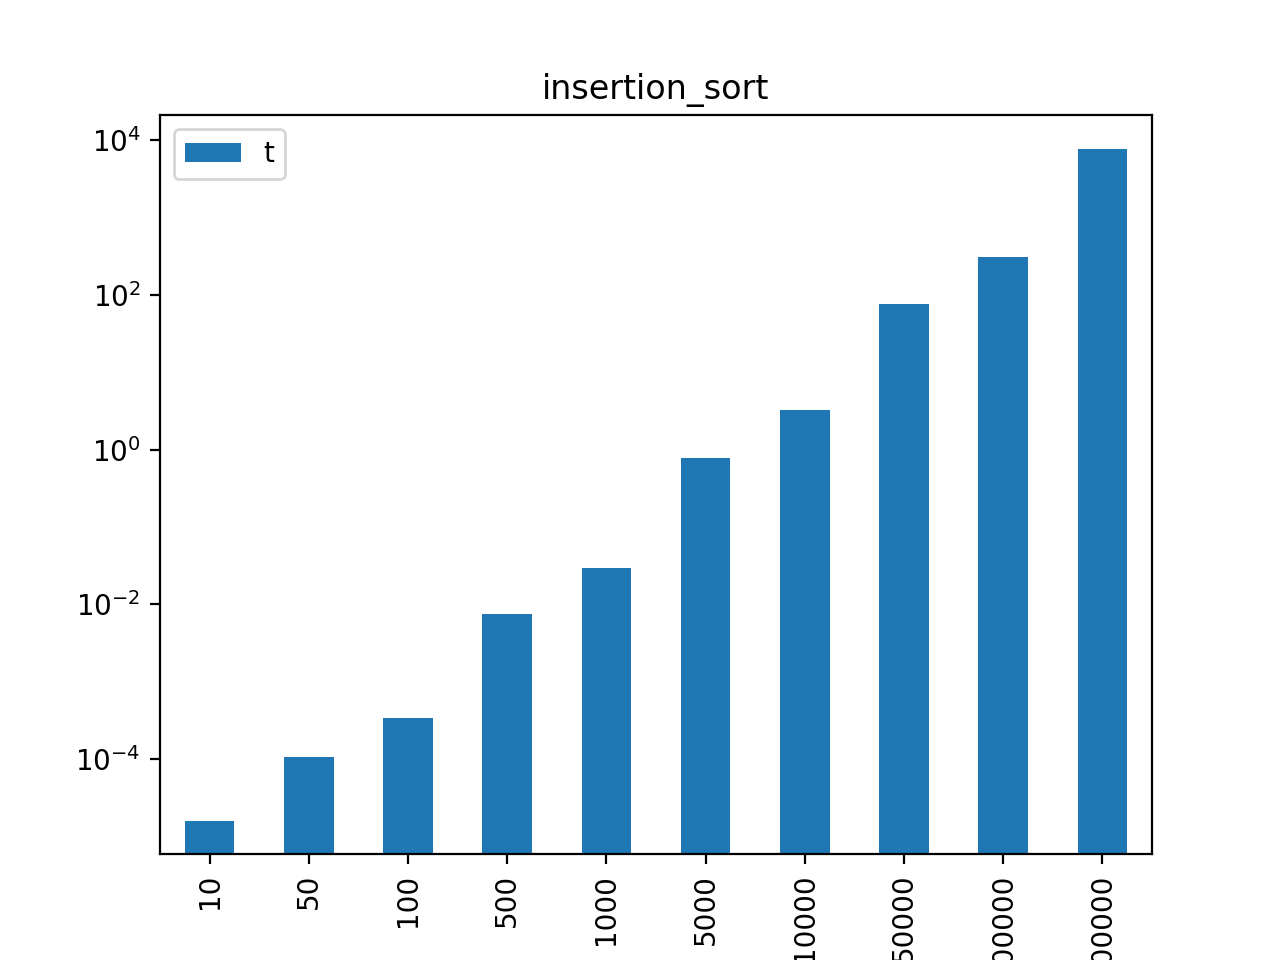
\includegraphics[width=8cm]{insertion_sort_r.png}	
			\end{figure}
		
		
\pagebreak
\section{Sortowanie kopcem}
	\subsection{Opis}
		Jest to typ sortowania niestabilnego. Wykorzystuje ono do sortowania strukturę jaką jest kopiec, przez co można go w części porównać do sortowania przez wstawianie. Tak jak sortowanie przez wstawanie sortowanie kopcem dzieli zbiór na część posortowaną i nie posortowaną. Różnica polego na ty, iż zamiast - jak sortowanie przez wstawianie - wybierać zawsze ten sam element, np. lewy skrajny z zbioru nie posortowanego, wybiera element największy z zbioru nie posortowanego.
	\subsection{Złożoność czasowa}
		Złożoność czasową tego algorytmu można wyrazić jako
		\[
		O(n\log{n})
		\]
		Powstała ona jako
		\begin{gather*}
		O(\text{swtórz kopiec()}) = O(n) \\
		O(\text{napraw kopiec()}) = O(\log{n}) \\
		\end{gather*}
		\begin{multline*}
		O(\text{swtórz kopiec()}) + n * O(\text{napraw kopiec()}) = \\ O(n) + n * O(\log{n}) = \\ O(n) + O(n\log{n}) = \\ O( n + n\log{n}) = \\ O(n(1 + \log{n})) = \\ O(n\log{n})
		\end{multline*}
	\subsection{Efektywność algorytmu, a wstępne uporządkowania danych}
		\begin{figure}[H]
			\centering
			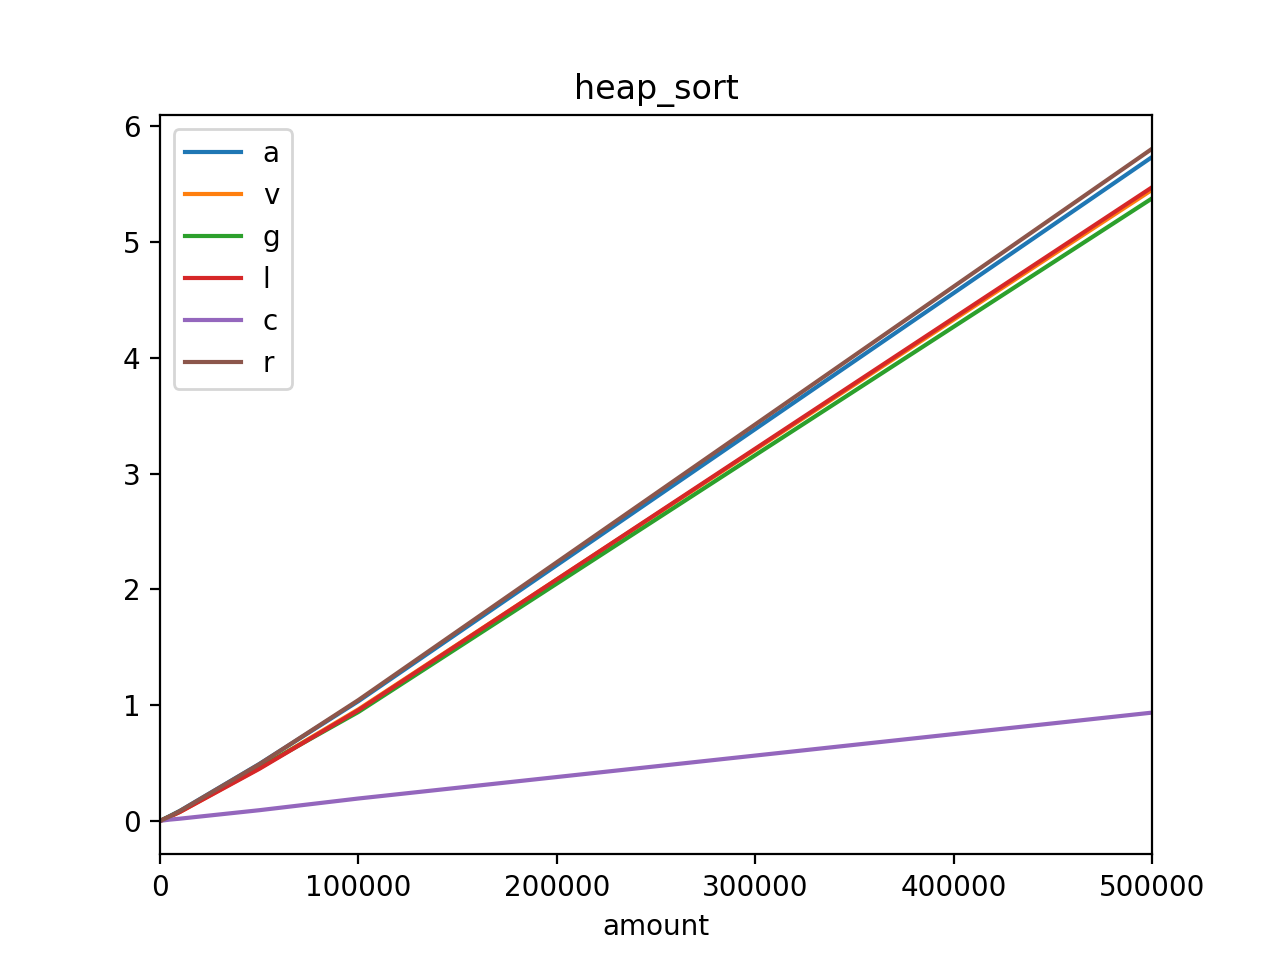
\includegraphics[width=8cm]{heap_sort_gather.png}	
		\end{figure}
	Sortowanie przy użyciu kopca nie jest wrażliwe na to jak są ułożone dane wejściowe. Jest to spowodowane, tym że złożoność czasowa powstaje w wyniku tworzenia i odbudowywania kopca, która odnotowywuje bardzo małe zmiany ze względu na to jak są ułożone dane. Jedynym znaczącym wyjątkiem jest przypadek w którym zbiór wymagający sortowanie składa się z tych samych elementów. Znaczące przyspieszenie uzyskuję się w wyniku skrócenia procedury odpowiedzialnej za odbudowę kopca, której złożoność spade z $ O(\log{n}) $ do $ O(1) $, w wyniku czego algorytm sortowania staje się liniowy
		\subsubsection{Uporządkowanie rosnąco-malejące}
		\begin{figure}[H]
			\centering
			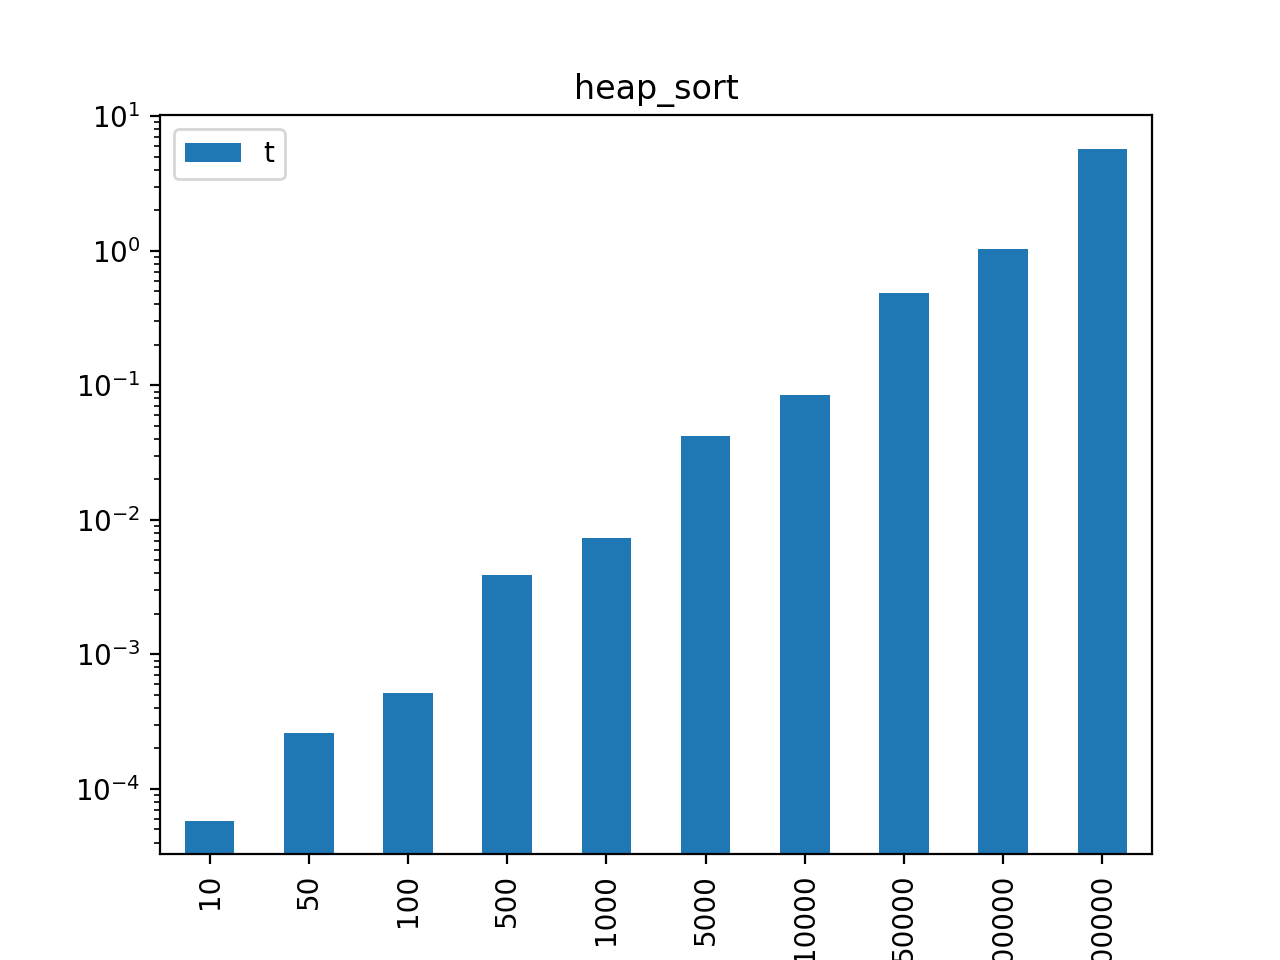
\includegraphics[width=8cm]{heap_sort_a.png}	
		\end{figure}
		\subsubsection{Uporządkowanie malejąco-rosnące}
		\begin{figure}[H]
			\centering
			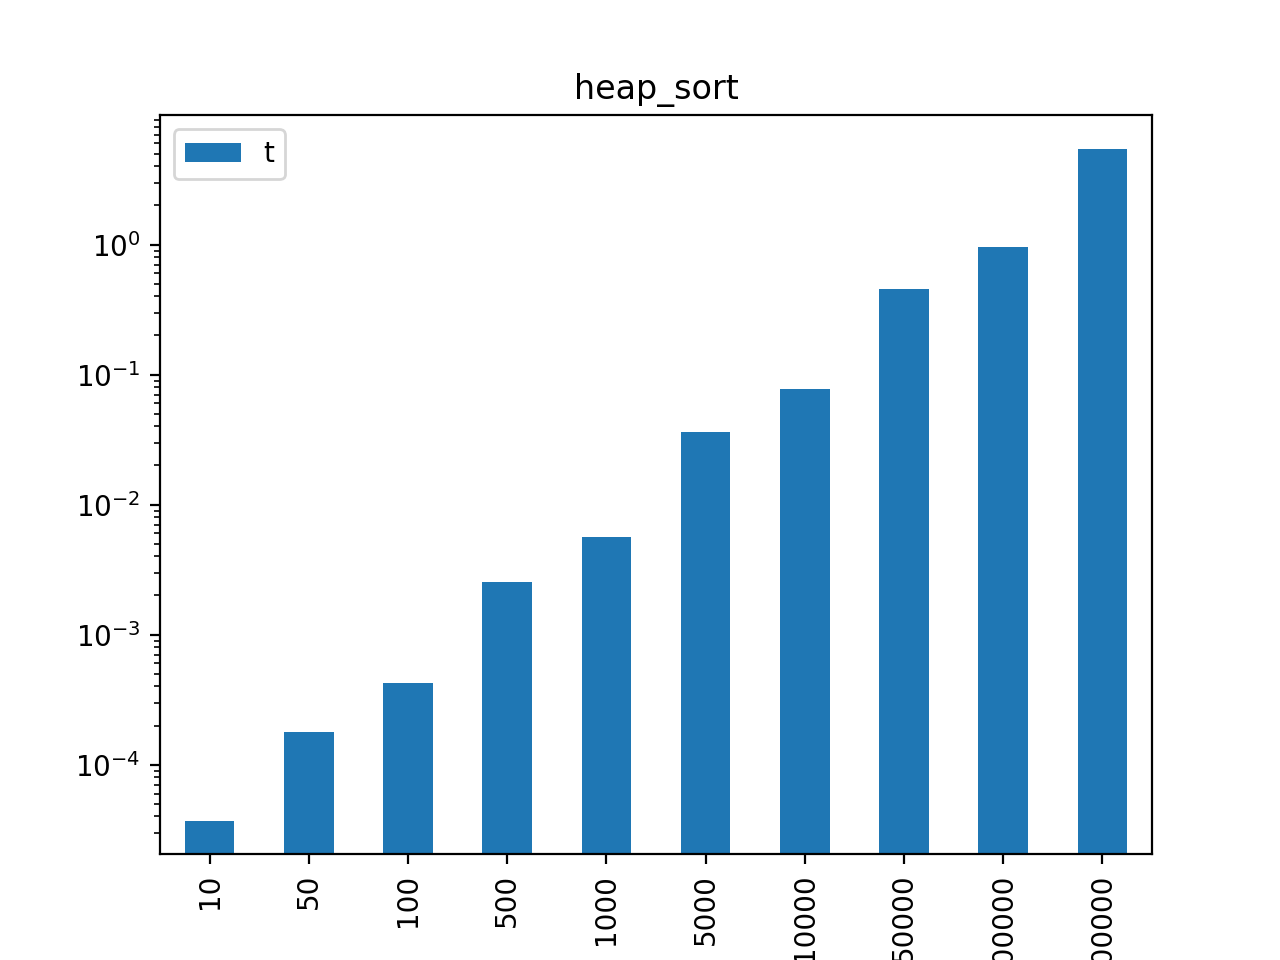
\includegraphics[width=8cm]{heap_sort_v.png}	
		\end{figure}
		\subsubsection{Uporządkowanie rosnące}
		\begin{figure}[H]
			\centering
			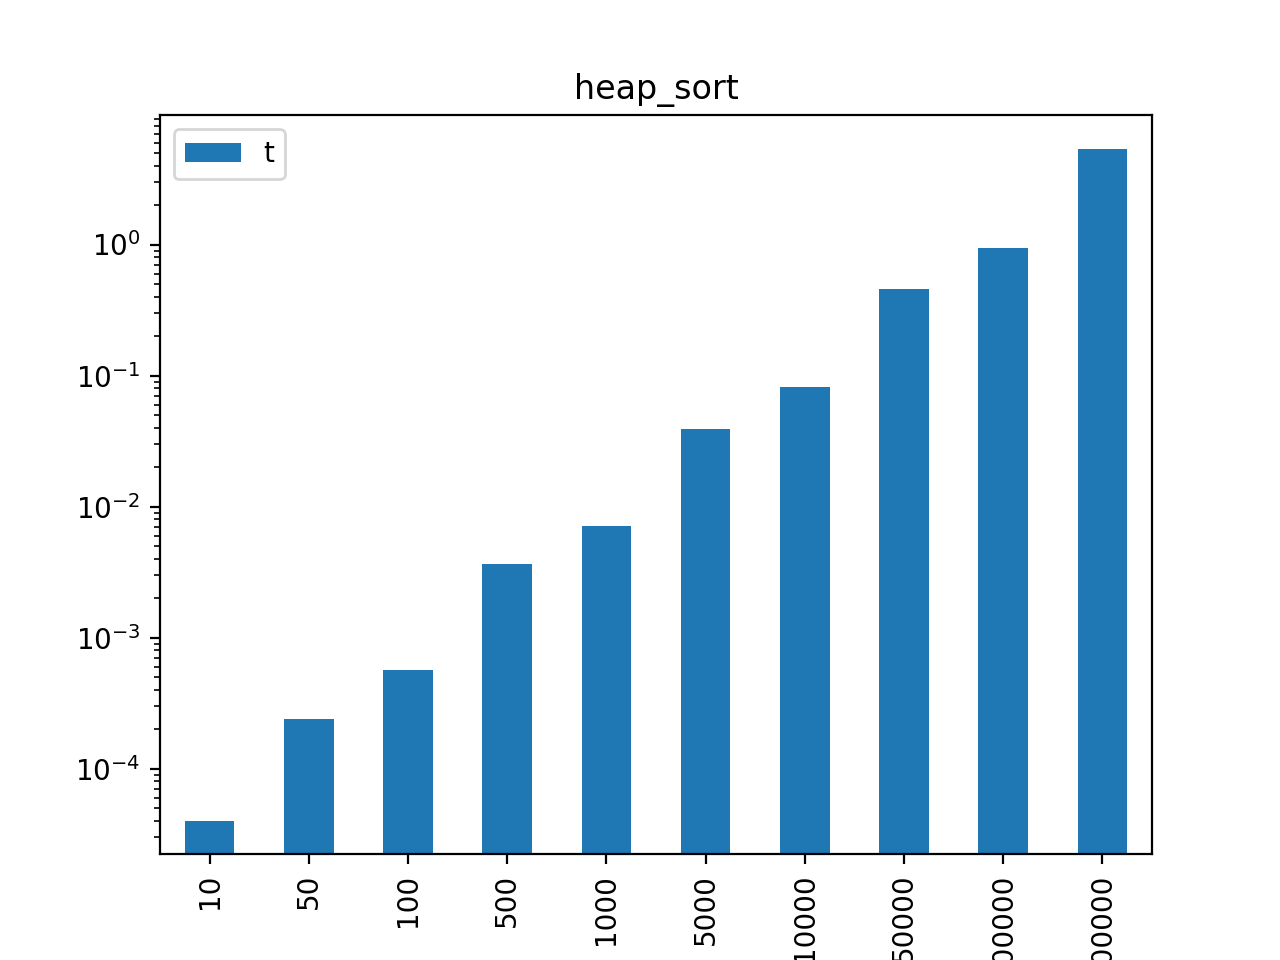
\includegraphics[width=8cm]{heap_sort_g.png}	
		\end{figure}
		\subsubsection{Uporządkowanie malejące}
		\begin{figure}[H]
			\centering
			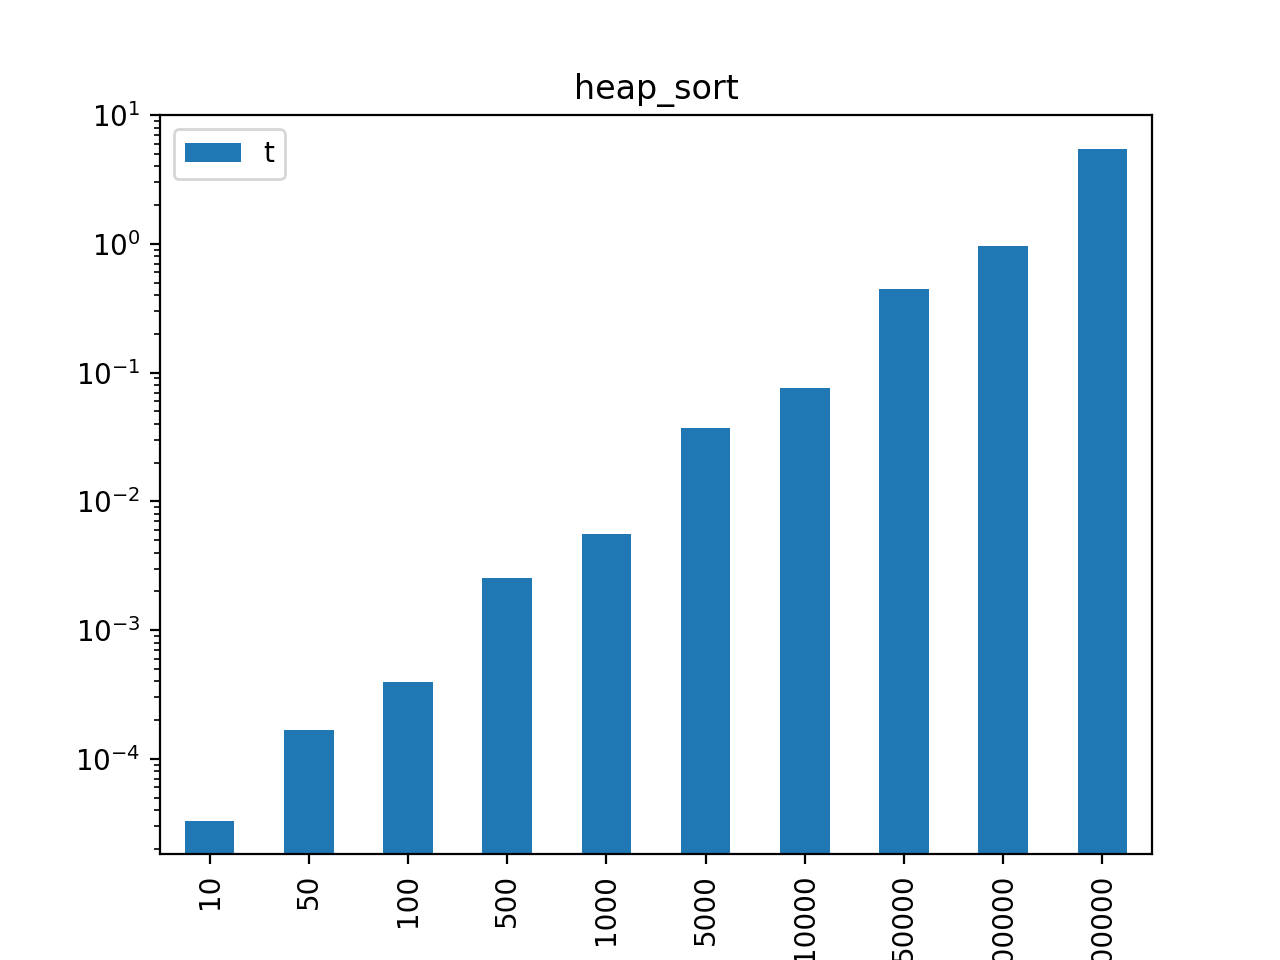
\includegraphics[width=8cm]{heap_sort_l.png}	
		\end{figure}
		\subsubsection{Wszystkie elementy są sobie równe}
		\begin{figure}[H]
			\centering
			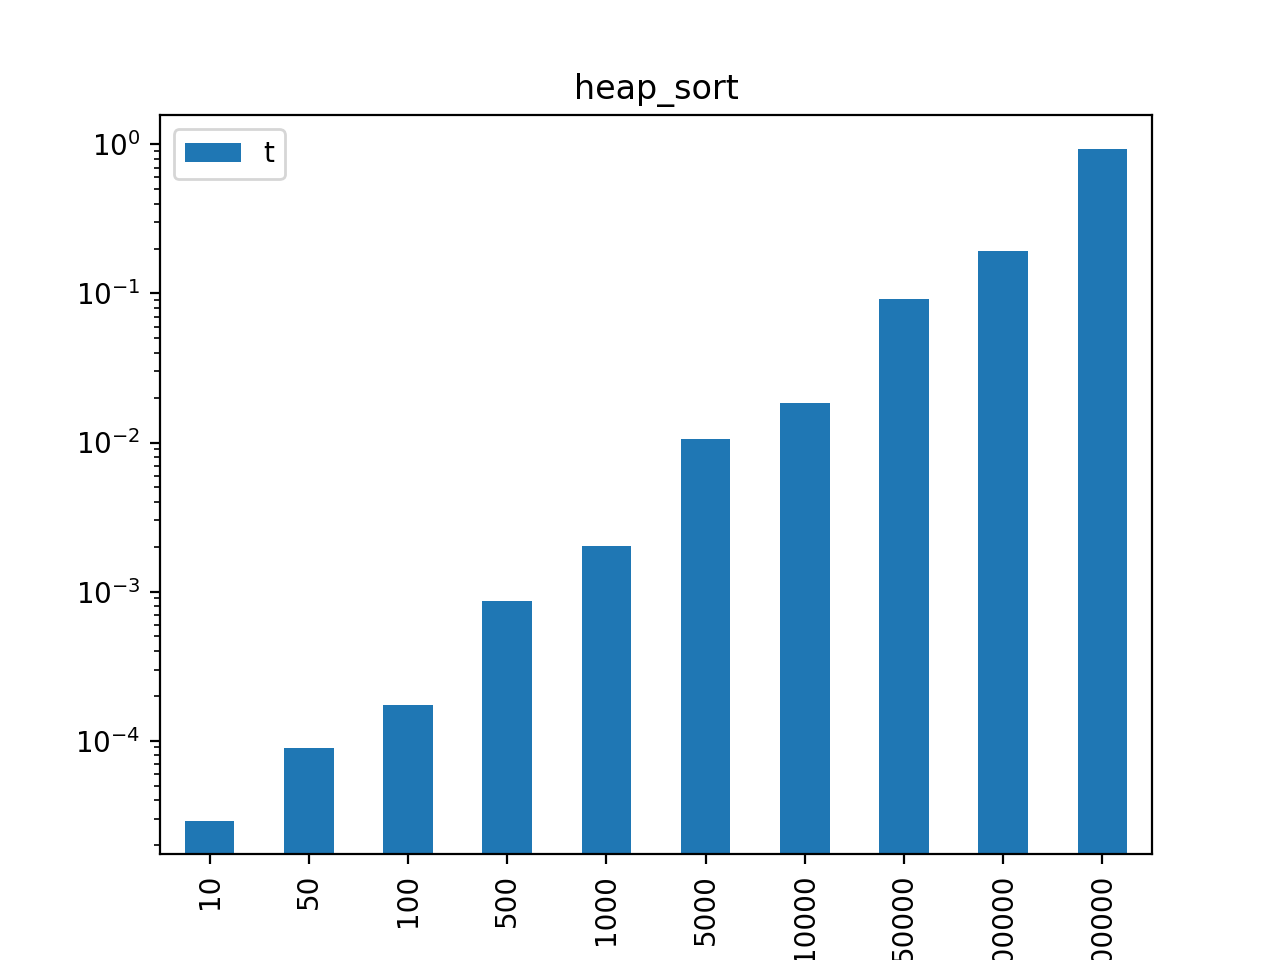
\includegraphics[width=8cm]{heap_sort_c.png}	
		\end{figure}
		\subsubsection{Brak wstępnego uporządkowania}
		\begin{figure}[H]
			\centering
			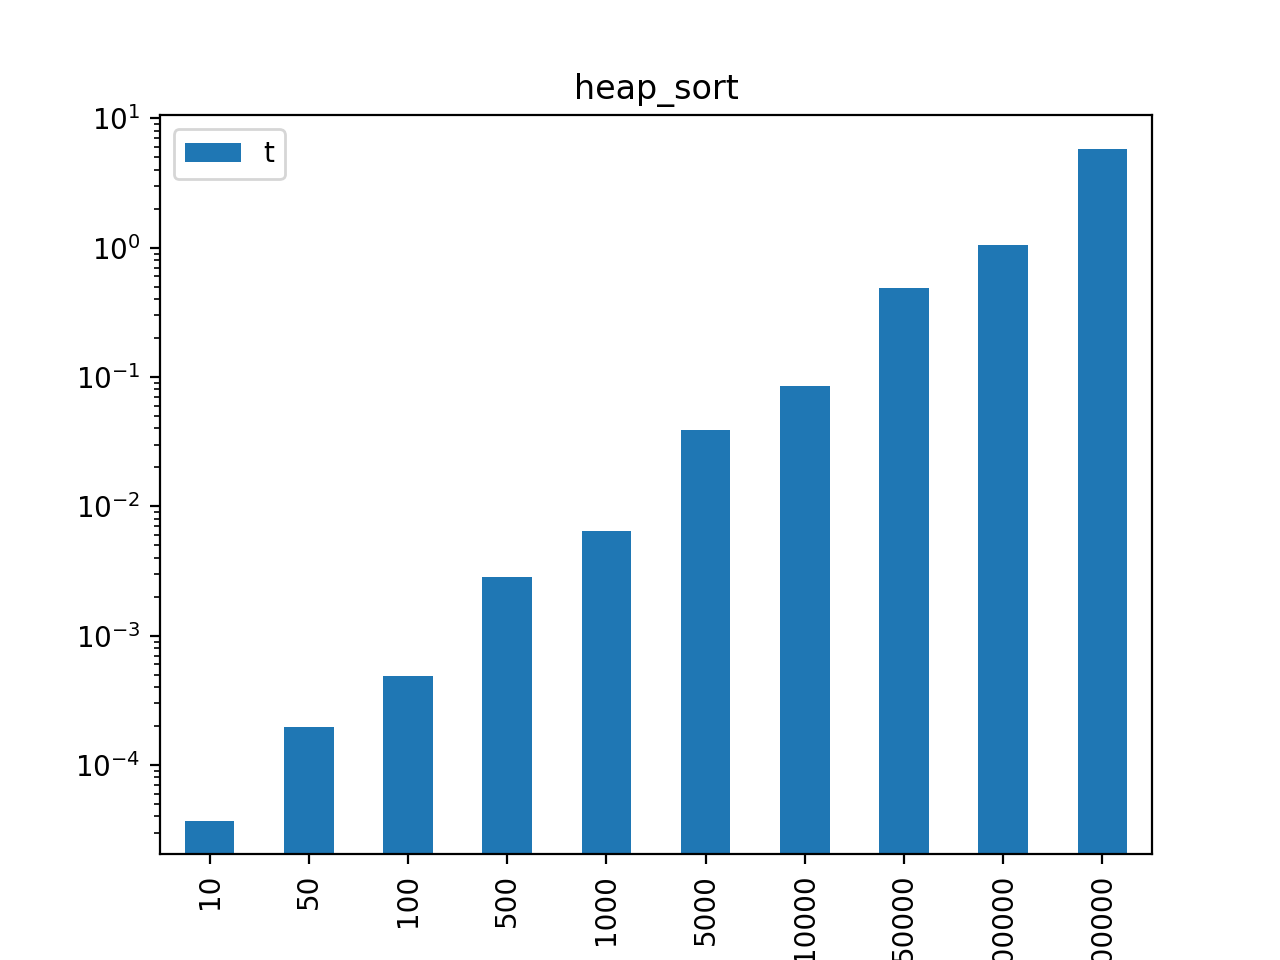
\includegraphics[width=8cm]{heap_sort_r.png}	
		\end{figure}
	
\pagebreak
\section{Sortowanie szybkie}
	\subsection{Opis}
		Jest to sortowanie niestabilne, używające metody dziel i zyciężaj (divide et impera). Polega ono na systematycznym podziale zbioru danych na dwa podzbiory, w idealnym przypadku równoliczne. Jeden z nich powinien zawierać elementy większe lub równe od pewnej, wcześniej wybranej wartości znajdującej się w sortowany zbiorze, a drugi mniejsze lub równe od tej wartości. W tym momencie należy powtórzyć wyżej wymienione kroki do momentu kiedy nie uzyskamy 1-ementowych lub 0-elementowych zbiorów. W tym momencie cały wejściowy zbiór powinien być posortowany.
	\subsection{Złożoność czasowa}
		Sortowanie szybkie charakteryzuje się złożonością czasową
		\[
		O(n\log{n})
		\]
		która wynika z rozumowania iż, pierwszy zbiór można podzielić na dwa podzbiory, każdy z tych dwóch podzbiorów można podzielić na dwa i tak dalej. Całą procedurę można zapisać jako drzewo binarne, w którym liście będą podzbiorami początkowego zbioru. Takie drzewo będzie miało $ \log{n} $ poziomów. Każdy z poziomów będzie wymagał conajwyżej n porównań, ponieważ, żaden z dwóch podzbiorów na tym samym poziomie nie ma części wspólnej. Ostatecznie dostajemy wzór 
		\begin{gather*}
			\text{ilość operacji} = \text{wysokość drzewa} *  \text{ilość sortowań na poziomie} \\  
			O(n\log{n})
		\end{gather*}
		jednak najgorszy przypadek zakłada złożoność 
		\[
		O(n^2)
		\]
		która bierze się z tego, że w wyniku podziału powstają dwa zbiory z których jeden jest jedno elementowy, co powoduje, że drzewo podziałów będzie drzewem o wysokości n, a nie $ \log{n} $
	\subsection{Efektywność algorytmu, a wstępne uporządkowania danych}
		Na wykres zaprezentowano porównanie algorytmów sortujących
		\begin{description}
			\item[quick sort right] sortowanie szybkie prawe, jako klucz użyty został skrajny prawy element, spośród wartości w sortowanym zbiorze
			
			\item[quick sort random] sortowanie szybkie losowe, jako klucz został użyty losowy klucz spośród wartości w sortowanym zbiorze
			
			\item[quick sort middle] sortowanie szybkie środkowe, jako klucz został użyty klucz będący na środku sortowanego zbioru wartości
			
			\item[quick sort left] sortowanie szybkie lewe, jako klucz został użyty skrajny lewy klucz spośród wartości z sortowanego zbioru wartości.
		\end{description}
		dodatkowo wszystkie algorytmy zostały wykonane na zbiorach o liczności 10000 elementów, a algorytm został zmodyfikowany do następującej postaci
		\begin{enumerate}
			\item jeżeli ilość elementów do posortowania jest mniejsza niż 2 to zwróc tablicę jaką otrzymałeś, jeśli nie to
			\item podziel wejściową tablicę na trzy inne tablice, tak aby: w jednej były elementy mniejsze od klucza, w drugiej elementy równe kluczowi, a w trzeciej elementy większe od klucza
			\item uruchom algorytm dla pierwszej tablicy
			\item uruchom algorytm dla trzeciej tablicy
		\end{enumerate}
		taka zmiana pozwoliła na zmiejszenie złożoności dla przypadku w którym wszystkie elementy zbioru sortowanego są równe
		\subsubsection{Uporządkowanie rosnąco-malejące}
		\begin{figure}[H]
			\centering
			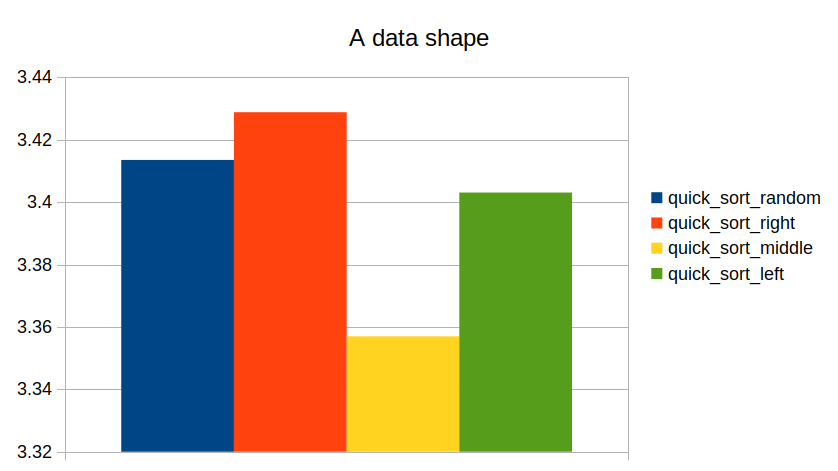
\includegraphics[width=8cm]{quick_sort_a.png}	
		\end{figure}
		W przypadku takiego ułożenia danych algorytmy częściej niż w przypadku gdy dane nie miały żadnego wstępnego uporządkowania, wybierały wartości największe lub najmniejsze w zbiorze. Objawiło się to wydłużeniem czasu w jakim się wykonywały.
		\subsubsection{Uporządkowanie malejąco-rosnące}
		\begin{figure}[H]
			\centering
			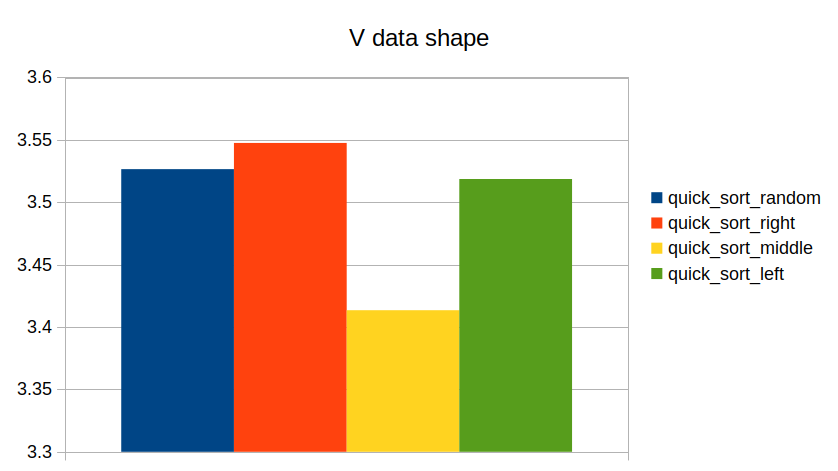
\includegraphics[width=8cm]{quick_sort_v.png}	
		\end{figure}
		Przypadek takiego uporządkowania danych wejściowych jest analogiczny do wcześniej analizowanego
		\subsubsection{Uporządkowanie rosnące}
		\begin{figure}[H]
			\centering
			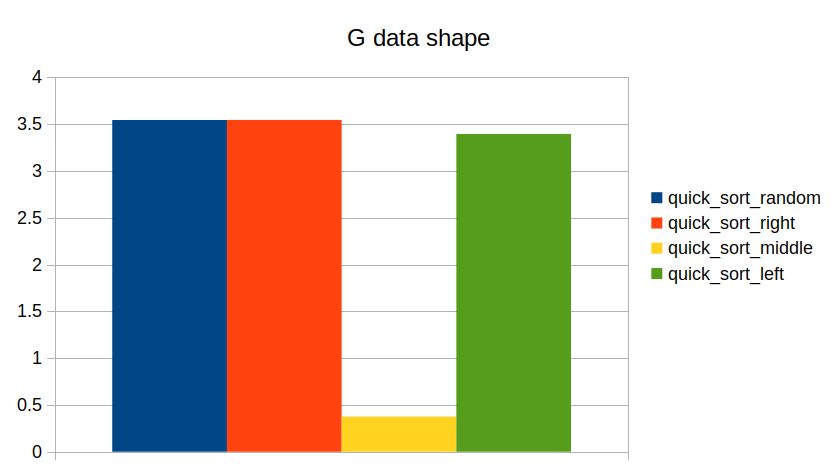
\includegraphics[width=8cm]{quick_sort_g.png}	
		\end{figure}
		Dane, uporządkowane w sposób rosnący wymuszają na prawie wszystkich algorytmach wybór ekstremów. Sytuacja jest inna dla algorytmu, wybierającego klucz jako element środkowy. Ten algorytm wykonuje się najszybciej, ponieważ często wybiera wartości będące medianą, a to powoduje, że przy każdorazowym podziale zbioru elementów sortowanych jest on dzielony na dwie równe części.
		\subsubsection{Uporządkowanie malejące}
		\begin{figure}[H]
			\centering
			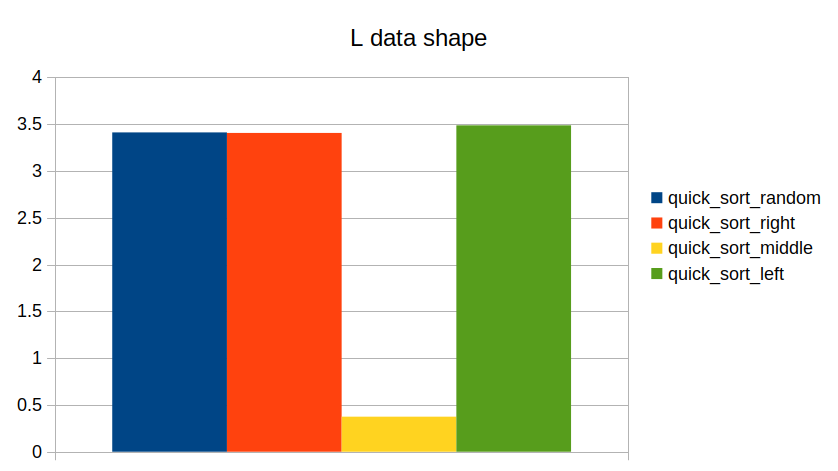
\includegraphics[width=8cm]{quick_sort_l.png}	
		\end{figure}
		Sytuacja dla tego typu uporządkowania danych wejściowych jest analogiczna do przypadku poprzedniego
		\subsubsection{Wszystkie elementy są sobie równe}
		\begin{figure}[H]
			\centering
			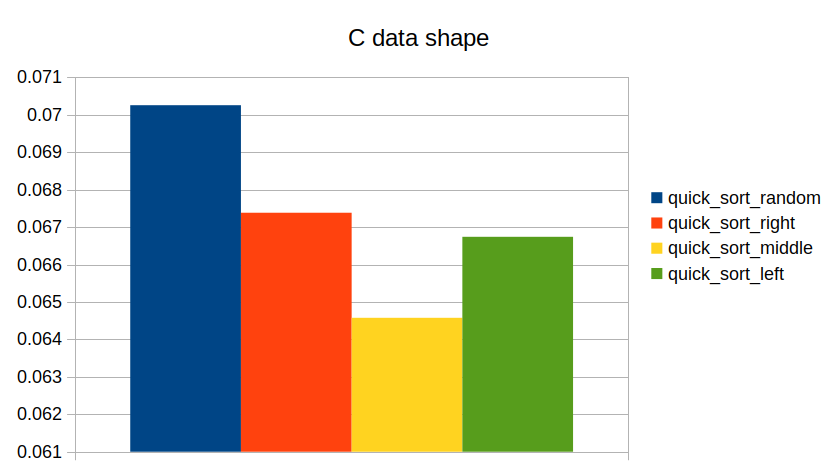
\includegraphics[width=8cm]{quick_sort_c.png}	
		\end{figure}
		Wszystkie algorytmy wykonują się o wiele szybciej, ponieważ już w pierwszym kroku przepisują do tablicy z elementami równymi kluczowi, wszytkie dane do posortowanie i kolejne wywołania funkcji sortującej kończą rekurencję oraz sortowanie. W takim wypadku sortowanie posiada złożoność liniową
		\subsubsection{Brak wstępnego uporządkowania}
		\begin{figure}[H]
			\centering
			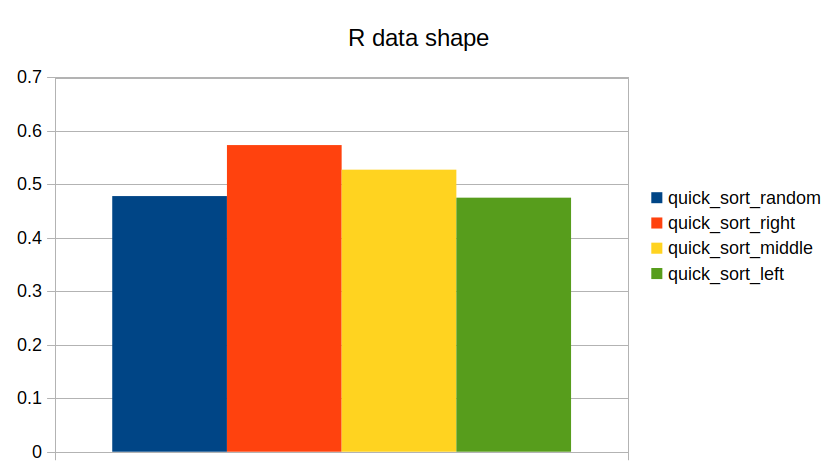
\includegraphics[width=8cm]{quick_sort_r.png}	
		\end{figure}

\pagebreak
\section{Sortowanie Shella}
	\subsection{Opis}
		Jest to rodaj sortowania niestabilnego w miejscu. Jest to rodzaj sortowania przez wstawianie, jednak z tą różnicą, że najpierw sortowane między sobą są elementy oddalone o pewną ustaloną odległość między sobą. Później ta odległości zostaje zmniejszana i elementy znowu zostają posortowane między sobą. Cała procedura jest powtarzana, do momentu kiedy odległość nie osiągnie wartości jeden. W tym momencie wykonuje się ostatnie sortowanie.
	\subsection{Złożoność czasowa}
		Złożoność algorytmu jest mocno powiązana z sekwencją zmian odległości między sortowanymi elementami. Najlepsze złożoności osiąga się dla sekwencji
		\[
		K = [x \in \mathbb{N}: 2^x - 1]
		\]
		wtedy złożoność można opisać jako
		\[
		O(n^{\frac{3}{2}})
		\]
		jednak jako najgorszą złożoność można przyjąć
		\[
		O(n^2)
		\]
	\subsection{Efektywność algorytmu, a wstępne uporządkowania danych}
		\begin{figure}[H]
			\centering
			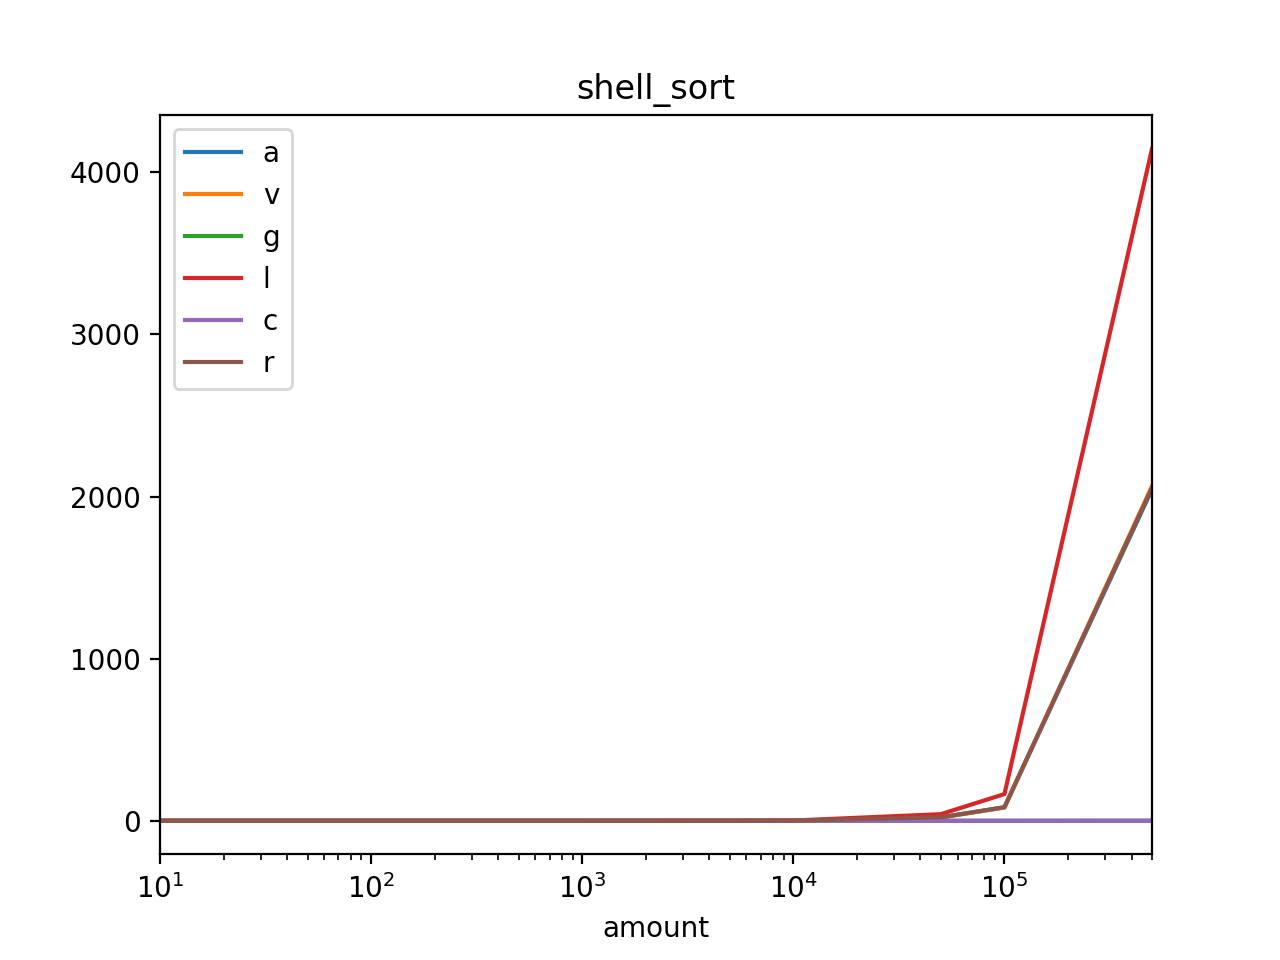
\includegraphics[width=8cm]{shell_sort_gather.png}	
		\end{figure}
		Na wykresach zastosowano skalę logarytmiczną, ze względu na duże zmiany w czasie potrzebnym na wykonanie algorytmów.
		Podczas sortowania wykorzystano serie $ K = [1923, 851, 323, 178, 53, 23, 7, 2, 1]] $, która spowodowała, że średnia złożoność wyniosła $ O(n^\frac{3}{2})$
		\subsubsection{Uporządkowanie rosnąco-malejące}
		\begin{figure}[H]
			\centering
			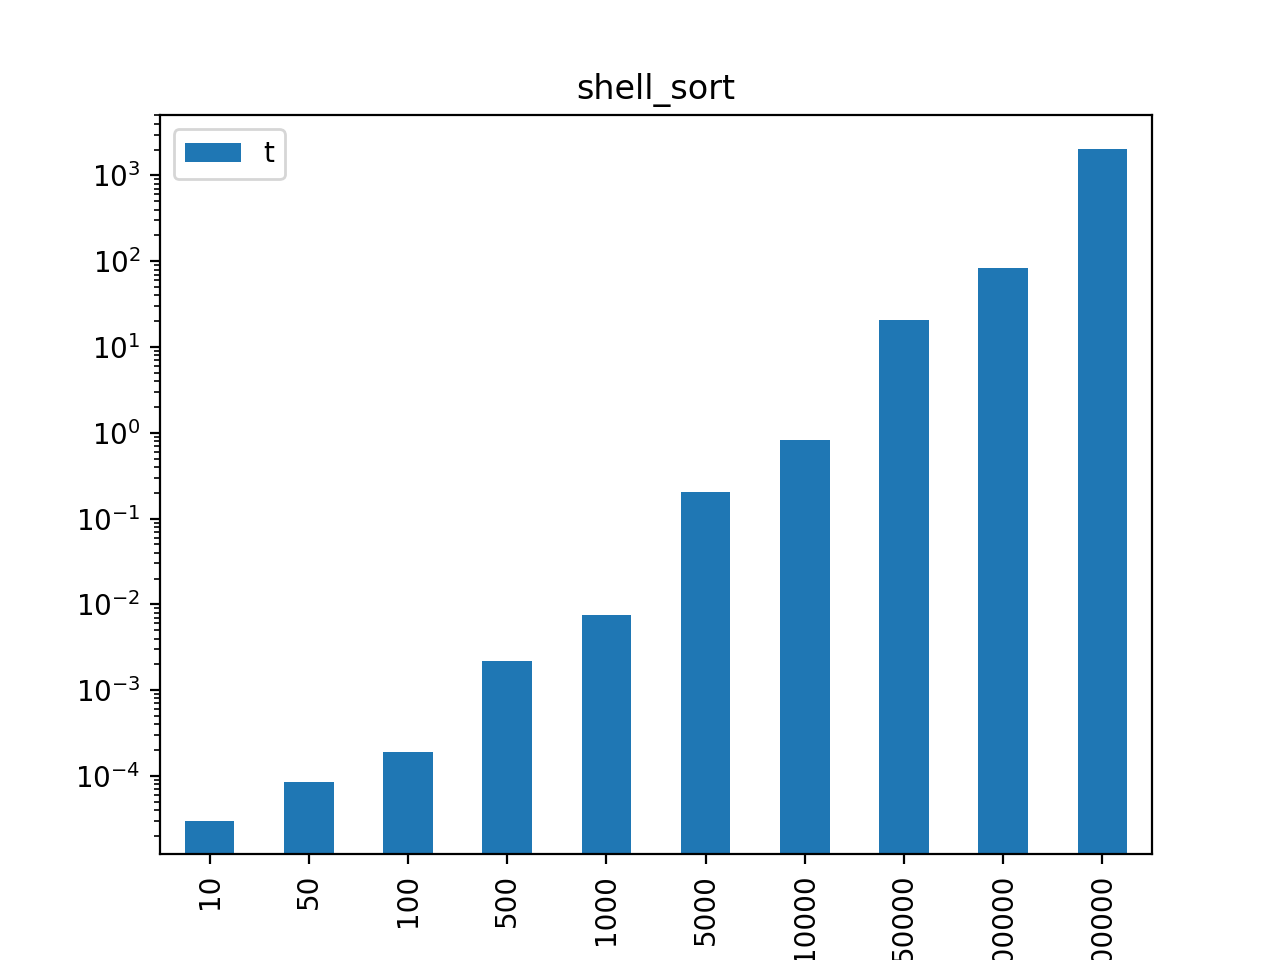
\includegraphics[width=8cm]{shell_sort_a.png}	
		\end{figure}
		Wykonanie algorytmu zajęło mniej więcej połowe czasu potrzebnego na wykonanie porządkowania zbioru ułożonego w sposób malejący. Stało się tak ponieważ tylko druga część zbioru wymagała sortowania
		\subsubsection{Uporządkowanie malejąco-rosnące}
		\begin{figure}[H]
			\centering
			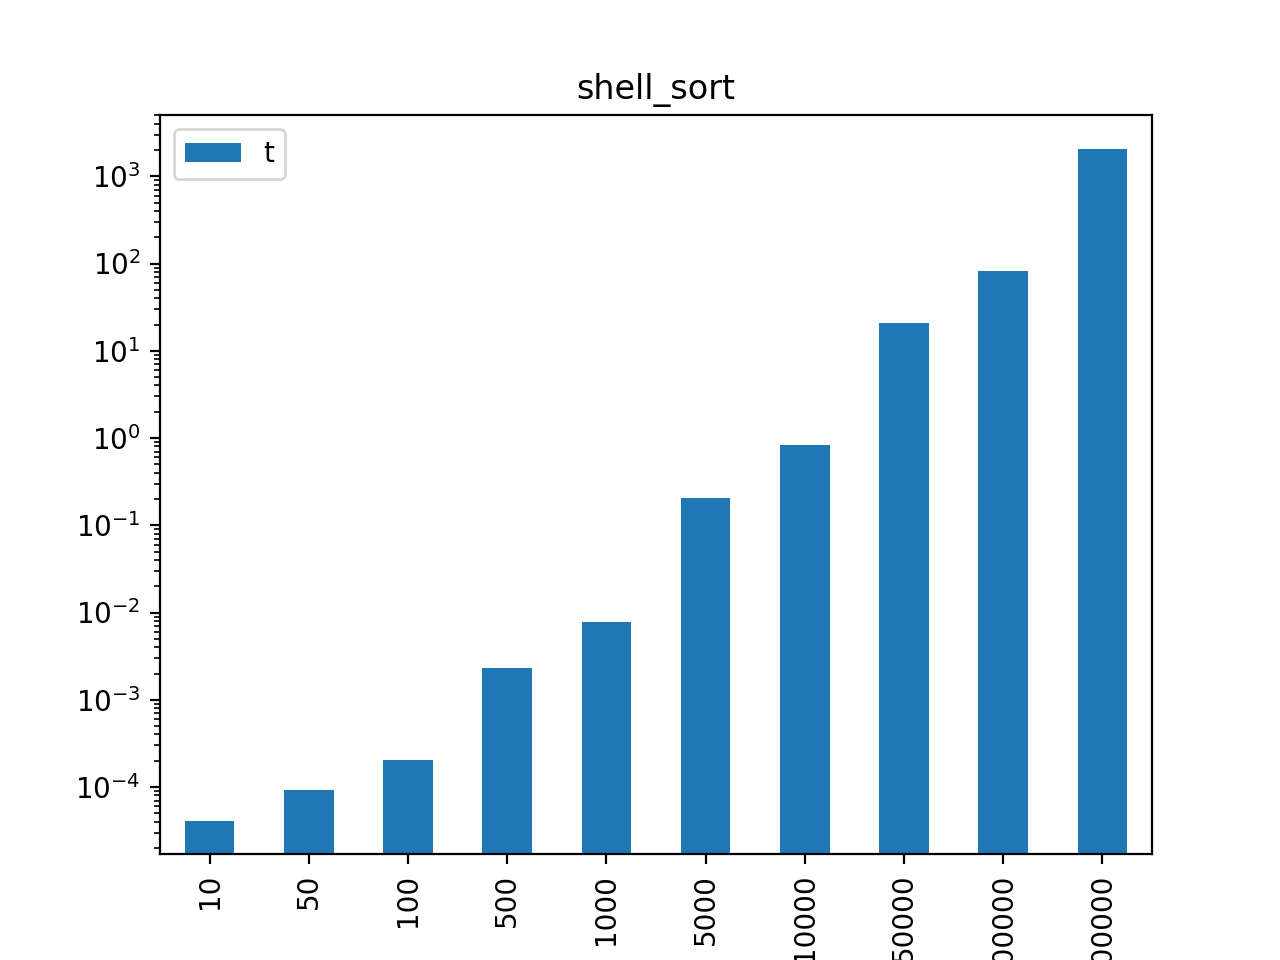
\includegraphics[width=8cm]{shell_sort_v.png}	
		\end{figure}
		Przypadek takiego ułożenia danych jest analogiczny do ułożenia opisywanego powyżej
		\subsubsection{Uporządkowanie rosnące}
		\begin{figure}[H]
			\centering
			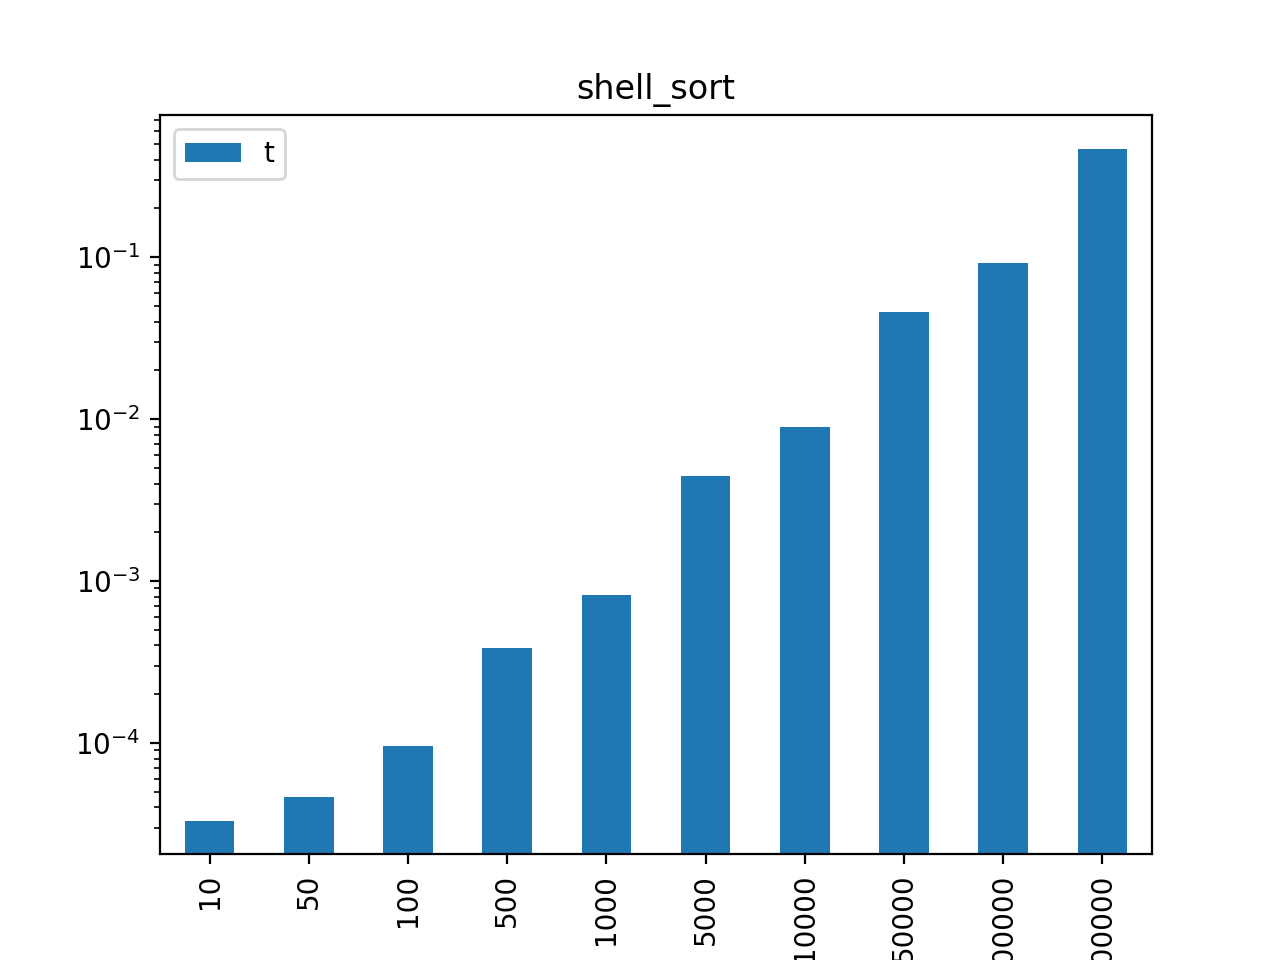
\includegraphics[width=8cm]{shell_sort_g.png}	
		\end{figure}
		Algorytm w przypadku danych wejściowych uporządkowanych rosnąco wykona się w ze złożonością zbliżoną do liniowej. Jest to spowodowane tym, że danych nie potrzeba zamieniać ze sobą miejscami. Jest sytuacja analogiczna jak w przypadku sortowania przez wstawianie dla takiego samego ułożenia danych
		\subsubsection{Uporządkowanie malejące}
		\begin{figure}[H]
			\centering
			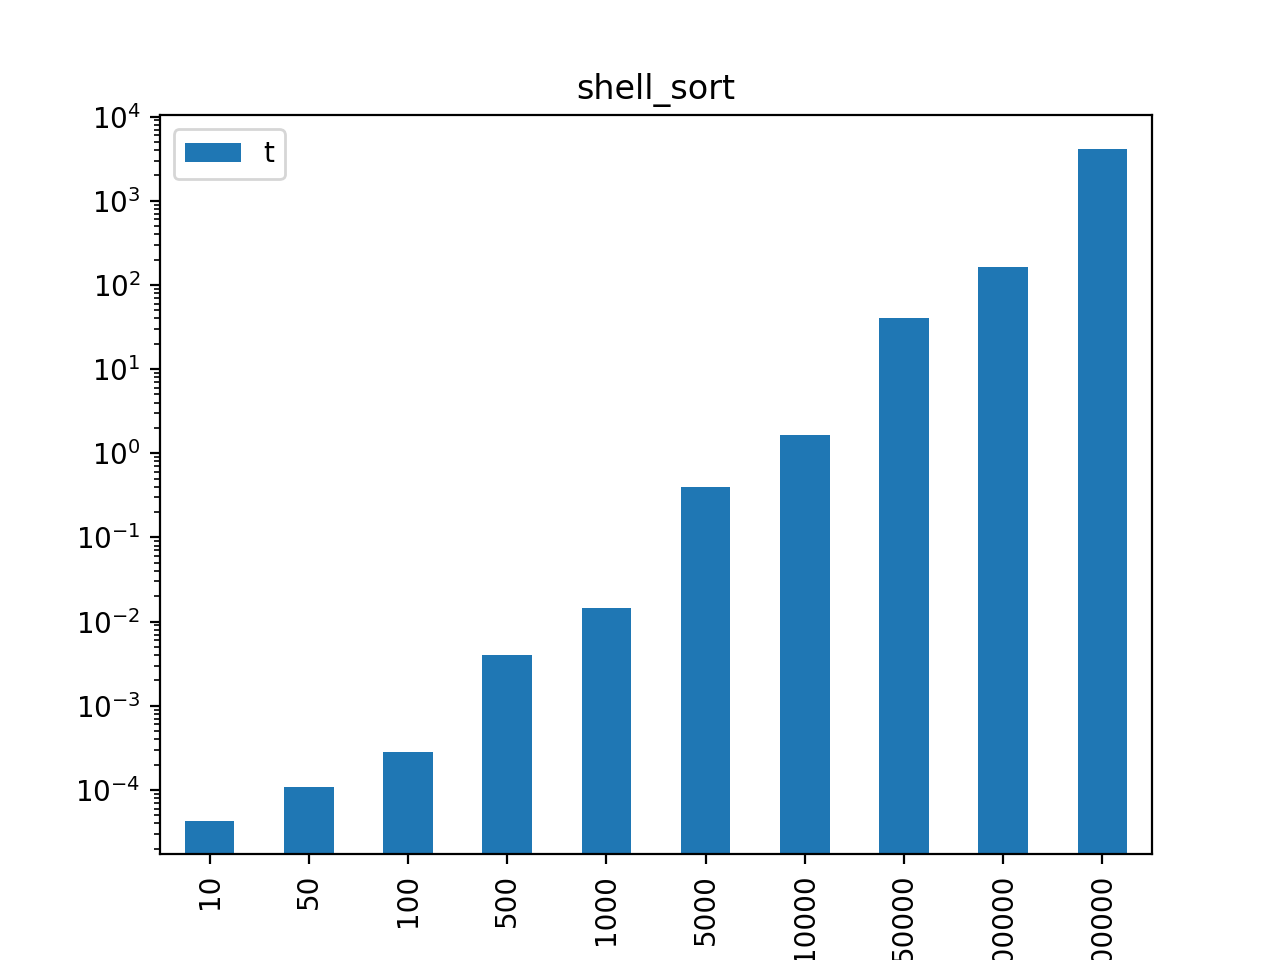
\includegraphics[width=8cm]{shell_sort_l.png}	
		\end{figure}
		Czas wykonania dla algorytmu jest najdłuższy, ponieważ, za każdym razem należy zmieniać ze sobą miejscami, większość elementów
		\subsubsection{Wszystkie elementy są sobie równe}
		\begin{figure}[H]
			\centering
			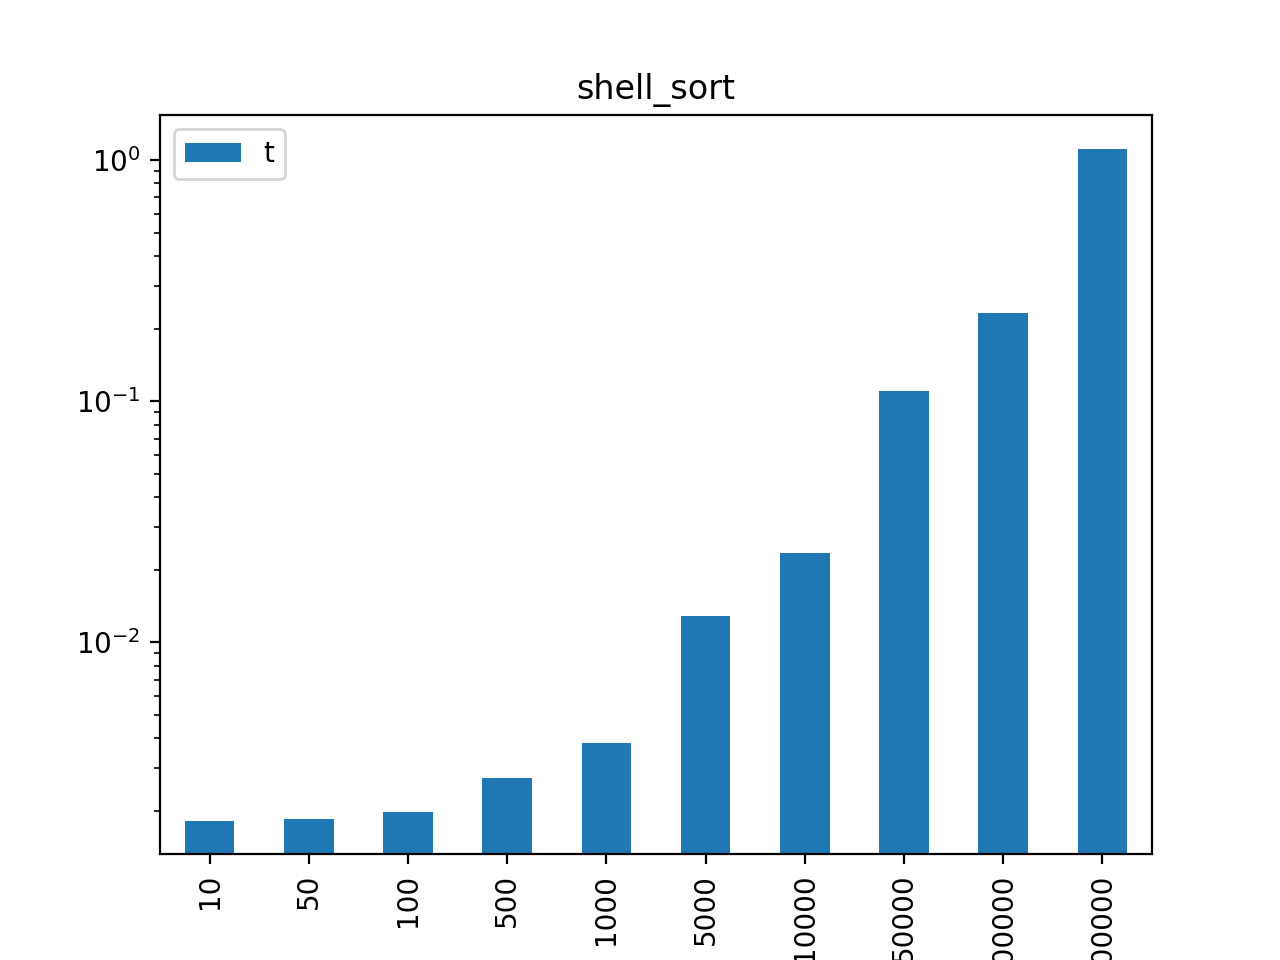
\includegraphics[width=8cm]{shell_sort_c.png}	
		\end{figure}
		Poprawnie zaimplementowny algortm wykona się w tym przypadku ze złożonościa, zbliżoną do liniowej, ponieważ, wszystkie elementy są ułożone na właściowych miejscach. Można tutaj szukać powiązania ze złożonością sortowania przez wstawianie
		\subsubsection{Brak wstępnego uporządkowania}
		\begin{figure}[H]
			\centering
			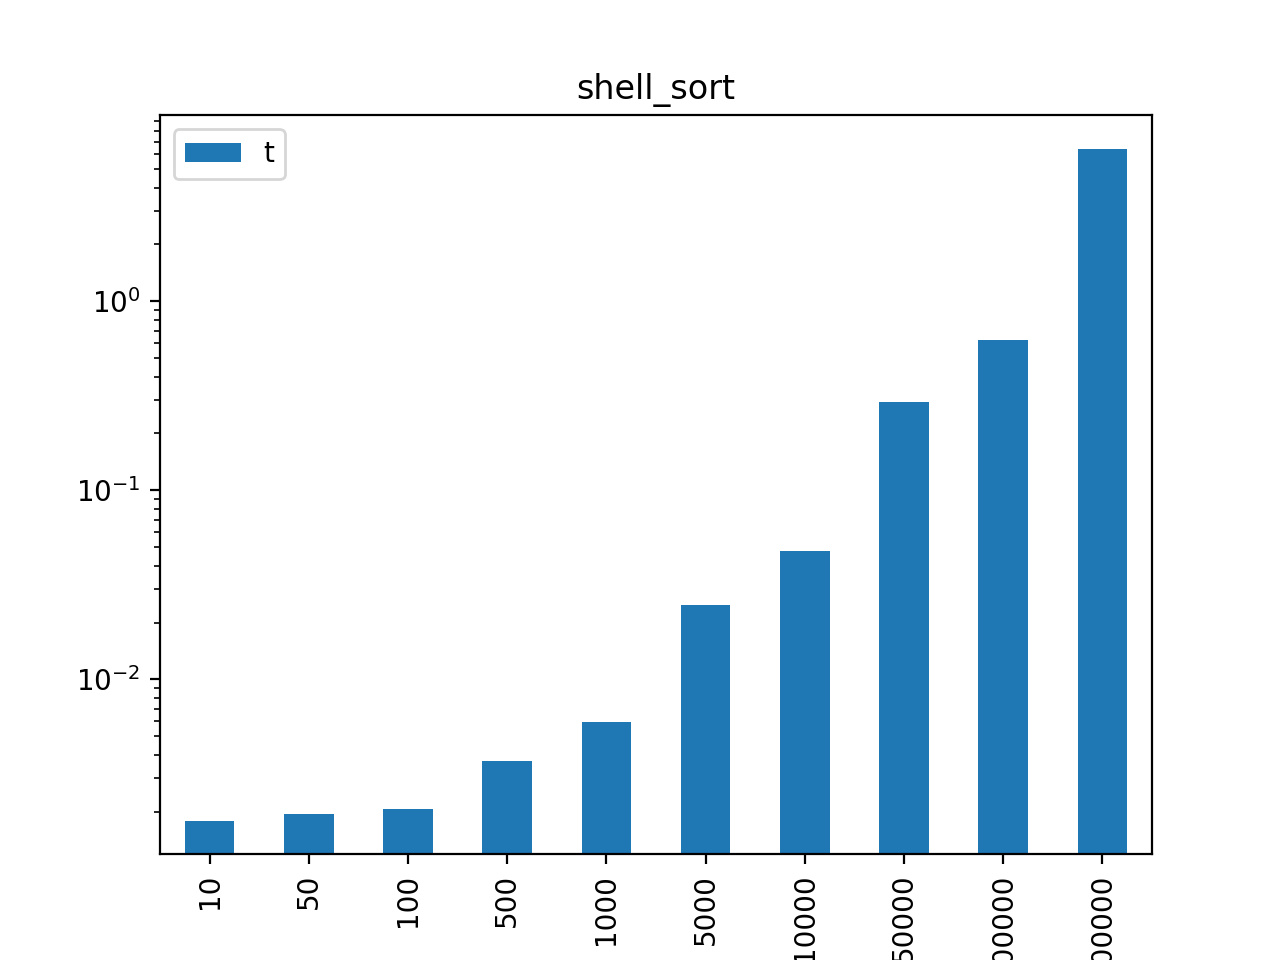
\includegraphics[width=8cm]{shell_sort_r.png}	
		\end{figure}


\pagebreak
\tableofcontents
\end{document}
